\documentclass[english]{exercisesheet}

\usepackage{mymath}
\usepackage{breqn}
\usepackage{graphicx}

\author{Daniel Strenger, Lorenzo Minneci}
\immatriculationnumber{01531211, 11939539}
\semester{SS 2020}
\subject{Machine Learning}
\sheetnumber{1}

\begin{document}
 \makedocumentheader
 \begin{nexercise}{Probability Refresher}
 \end{nexercise}
 \begin{solution}
 We calculate $\p(T=1,D=0)=\p(D=0)\p(T=1|D=0)=95\%\cdot1\%=0.95\%$,\\
 $\p(T=0,D=0)=\p(D=0)\p(T=0|D=0)=\p(D=0)(1-\p(T=1|D=0))=95\%\cdot99\%=94.05\%$,\\
 $\p(T=1,D=1)=\p(D=1)\p(T=1|D=1)=4\%\cdot20\%=0.8\%$,
\\
$\p(T=0,D=1)=\p(D=1)(1-\p(T=1|D=1))=4\%\cdot80\%=3.2\%$,\\
$\p(T=1,D=2)=\p(D=2)\p(T=1|D=2)=1\%\cdot98\%=0.98\%$,\\
$\p(T=0,D=2)=\p(D=2)(1-\p(T=1|D=2))=1\%\cdot2\%=0.02\%$,\\
$\p(T=1)=\p(T=1,D=0)+\p(T=1,D=1)+\p(T=1,D=2)=2.73\%$ (because the events $D=0,1,2$ are disjoint),\\
$\p(T=0)=1-p(T=1)=97.27\%$.\\
This gives the table
  \begin{center}
\begin{tabular}{|l|l|l|l|l|}
\hline
 & healthy ($D=0$) &allergy ($D=1$)  &celiac ($D=2$)  &$p(T_i)$  \\ \hline
pos. ($T=1$)&$0.95\%$  & $0.8\%$ & $0.98\%$ & $2.73\%$ \\ \hline
 neg. ($T=0$)& $94.05\%$ &$3.2\%$  & $0.02\%$ & $97.27\%$ \\ \hline
 $p(D_i)$& $95\%$ & $4\%$ & $1\%$¸ &  \\ \hline
\end{tabular}
\end{center}
 \end{solution}
 
 
\begin{nexercise}{Mutual Information}
\end{nexercise}
\begin{solution}
 1. We have
 \begin{equation*}
  \Sigma^{-1}=\frac{1}{\det(\Sigma)} \begin{pmatrix}
                                    \sigma^2&-\alpha\sigma^2\\
                                      -\alpha\sigma^2& \sigma^2
                                     \end{pmatrix}
    =\frac{1}{\sigma^4-\alpha^2\sigma^4} \begin{pmatrix}
                                    \sigma^2&-\alpha\sigma^2\\
                                      -\alpha\sigma^2& \sigma^2
                                     \end{pmatrix}
 \end{equation*}
\begin{equation*}
 \Rightarrow (x,y)
             \Sigma^{-1}\begin{pmatrix}
                         x\\y
                        \end{pmatrix}
=\frac{1}{\sigma^4-\alpha^2\sigma^4} (x,y)\begin{pmatrix}
                                    \sigma^2&-\alpha\sigma^2\\
                                      -\alpha\sigma^2& \sigma^2
                                     \end{pmatrix}\begin{pmatrix}
                                     x\\y
                                     \end{pmatrix}
=\frac{1}{\sigma^4(1-\alpha^2)}(x^2+y^2-2xy\alpha)
\end{equation*}
\begin{equation*}
 \Rightarrow p_{X,Y}(x,y)=\frac{1}{2\pi\sigma^2\sqrt{1-\alpha^2}}\exp\left(-\frac{1}{2\sigma^2(1-\alpha^2)}(x^2+y^2-2xy\alpha)\right)
\end{equation*}
The one dimensional marginal distributions of a multivariate normal distribution are univariate normal distributions,
\begin{equation*}
 p_X(x)=\frac{1}{\sqrt{2\pi\sigma^2}}\exp\left(-\frac{x^2}{2\sigma^2}\right),~p_Y(y)=\frac{1}{\sqrt{2\pi\sigma^2}}\exp\left(-\frac{y^2}{2\sigma^2}\right).
\end{equation*}
From that we get
\begin{equation*}
 I(X;Y)=\int_\R\int_\R p_{X,Y}(x,y)\log\left(\frac{p_{X,Y}(x,y)}{p_X(x)p_Y(y)}\right) dy dx
 \end{equation*}
 \begin{equation*}
 =\int_\R\int_\R p_{X,Y}(x,y)\log\left(\dfrac{\frac{1}{2\pi\sigma^2\sqrt{1-\alpha^2}}\exp\left(-\frac{1}{2\sigma^2(1-\alpha^2)}(x^2+y^2-2xy\alpha)\right)}{\frac{1}{\sqrt{2\pi\sigma^2}}\exp\left(-\frac{x^2}{2\sigma^2}\right)\cdot\frac{1}{\sqrt{2\pi\sigma^2}}\exp\left(-\frac{y^2}{2\sigma^2}\right)}\right)dydx
\end{equation*}
\begin{equation*}
 =\int_\R\int_\R p_{X,Y}(x,y)\left(\log\left(\frac{1}{\sqrt{1-\alpha^2}}\right)-\frac{x^2+y^2-2xy\alpha}{2\sigma^2(1-\alpha^2)}+\frac{x^2}{2\sigma^2}+\frac{y^2}{2\sigma^2}\right)dydx
\end{equation*}
\begin{align*}
 =-\frac{1}{2}\log(1-\alpha^2) \underbrace{\int_\R\int_\R p_{X,Y}(x,y)dydx}_{=1}\\
 -\int_R\int_R p_{X,Y}(x,y) \left(\frac{x^2+y^2-2xy\alpha}{2\sigma^2(1-\alpha^2)}-\frac{x^2(1-\alpha^2)}{2\sigma^2(1-\alpha^2)}-\frac{y^2(1-\alpha^2)}{2\sigma^2(1-\alpha^2)}\right)dydx
\end{align*}
\begin{equation*}
 =-\frac{1}{2}\log(1-\alpha^2)-\frac{\alpha}{1-\alpha^2}\int_\R\int_\R p_{X,Y}(x,y)\frac{\alpha x^2+\alpha y^2-2xy}{2\sigma^2}dydx
\end{equation*}
\begin{align*}
 =-\frac{1}{2}\log(1-\alpha^2)-\frac{\alpha}{1-\alpha^2}\left(\int_\R \alpha(x-0)^2\underbrace{\int_\R p_{X,Y}(x,y)dy}_{=p_X(x)}dx+\int_\R \alpha (y-0)^2\underbrace{\int_\R p_{X,Y}(x,y)dx}_{=p_Y(y)}dy\right.\\
 \left.-2\int_\R\int_\R (x-0)(y-0) p_{X,Y}(x,y) dydx\right)
\end{align*}
\begin{equation*}
 =-\frac{1}{2}\log(1-\alpha^2)-\frac{\alpha}{1-\alpha^2}\left(\alpha\int_\R (x-\mu_x)^2 p_X(x)dx+\alpha\int_\R (y-\mu_y)^2p_Y(y)dy-2\int_\R\int_\R (x-\mu_x)(y-\mu_y)p_{X,Y}(x,y)dydx\right)
\end{equation*}
\begin{equation*}
 =-\frac{1}{2}\log(1-\alpha^2)-\frac{\alpha}{1-\alpha^2}\left(\alpha\var(X)+\alpha\var(Y)-2\cov(X,Y)\right)=-\frac{1}{2}\log(1-\alpha^2)-\frac{\alpha}{1-\alpha^2}\left(\alpha\sigma^2+\alpha\sigma^2-2\alpha\sigma^2\right)
 \end{equation*}
 \begin{equation*}
 =-\frac{1}{2}\log(1-\alpha^2)
\end{equation*}
\par2. $I(X;Y)$ is strictly monotonously increasing in $\alpha^2$, so it is minimal for $\alpha^2=0\Leftrightarrow \alpha=0$, which corrsponds to the case that $X$ and $Y$ are independent. In this case $I(X;Y)=-\frac{1}{2}\log(1)=0$, which also reflects the independece.\\
The value of $I(X;Y)$ increases as $\alpha^2 \rightarrow 1 \Leftrightarrow \alpha \rightarrow \pm 1$. As $|\alpha|<1$ these values are never attained, but for $\alpha \rightarrow \pm 1$ the mutual information increases to infinity, so it is never maximal. The values $\alpha=\pm1$ would correspond to the (degenerate) cases that $Y$ is a function in $X$, i.e., if the value of $X$ is given, then also $Y$ is given.
\par3. The plots for $\sigma^2\in \lbrace 1,25,200\rbrace$ and $\alpha\in\lbrace 0, 0.5,0.9\rbrace$ are shown in figures 1-3.
\begin{figure}
 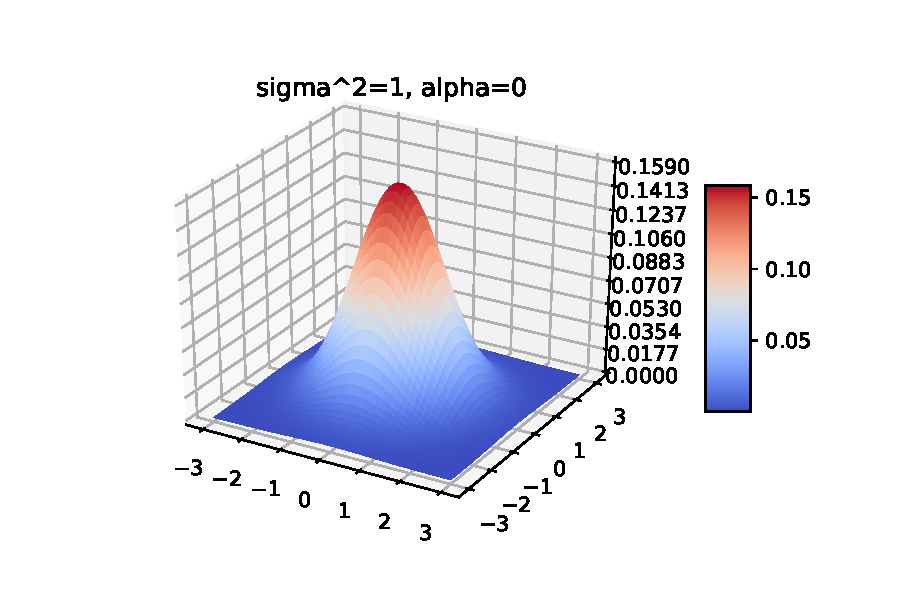
\includegraphics[width=0.5\textwidth]{images/plot-1-0-side.pdf} 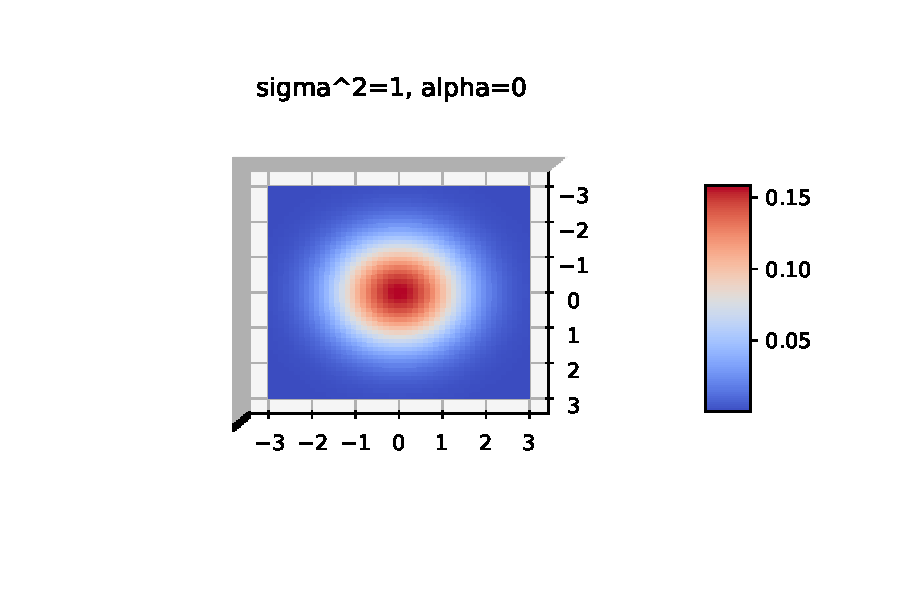
\includegraphics[width=0.5\textwidth]{images/plot-1-0-top.pdf}\\
 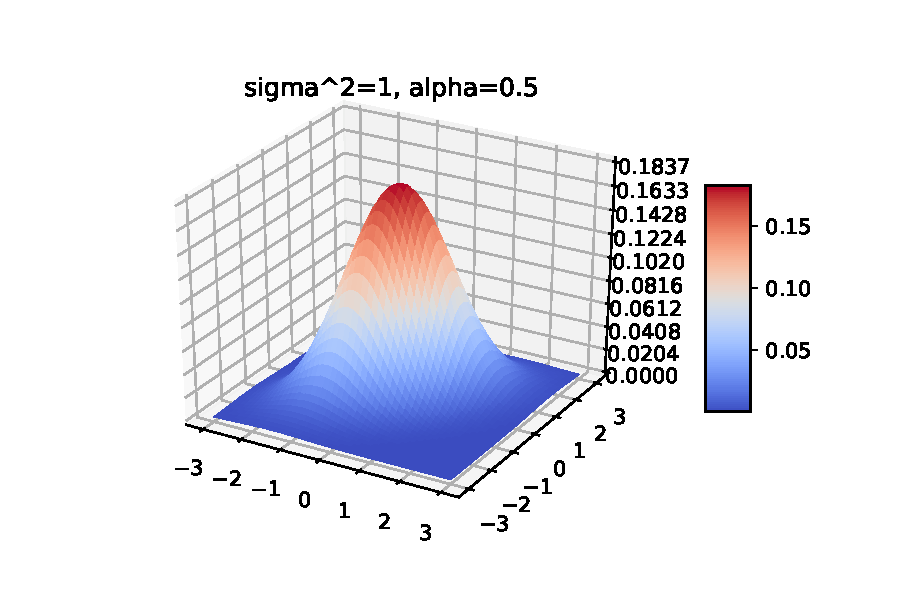
\includegraphics[width=0.5\textwidth]{images/plot-1-5-side.pdf} 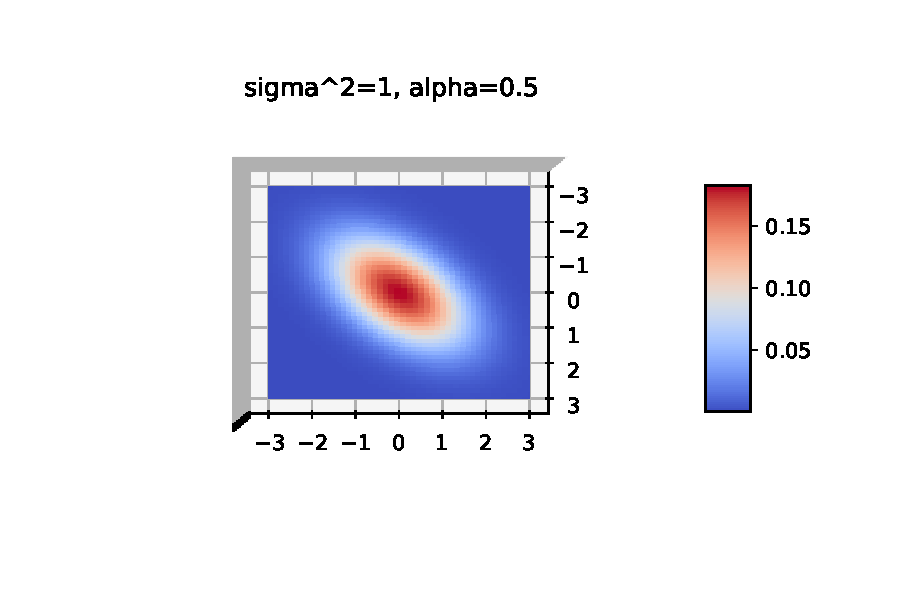
\includegraphics[width=0.5\textwidth]{images/plot-1-5-top.pdf}\\
 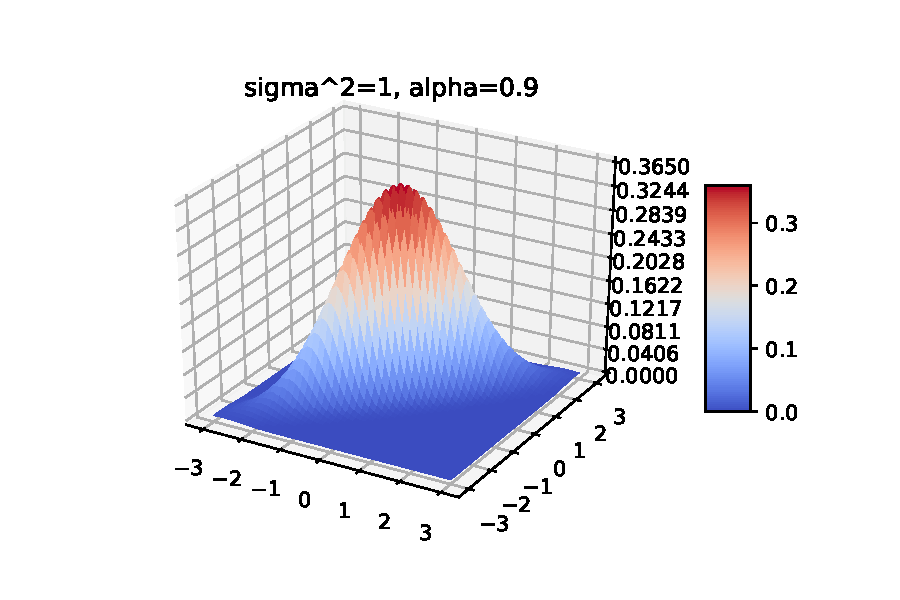
\includegraphics[width=0.5\textwidth]{images/plot-1-9-side.pdf} 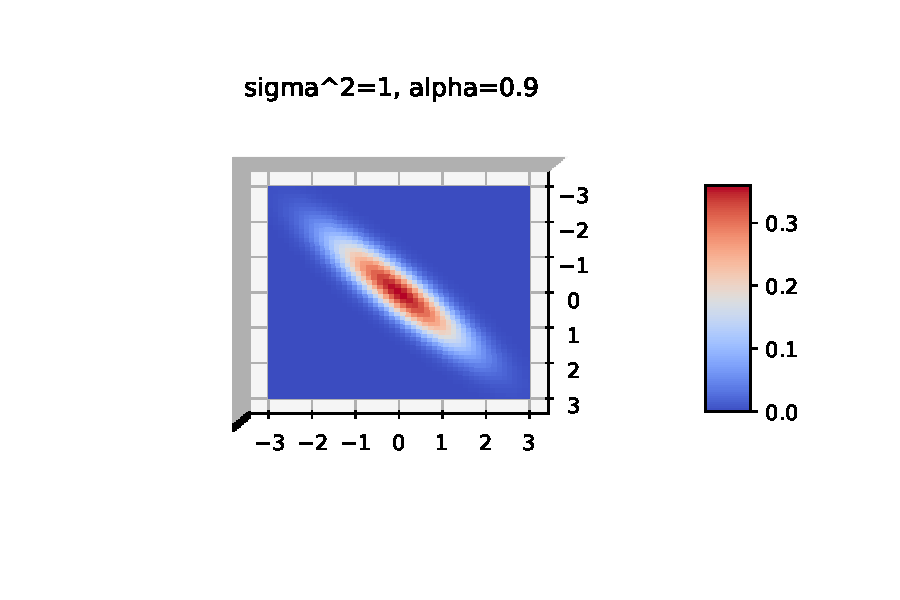
\includegraphics[width=0.5\textwidth]{images/plot-1-9-top.pdf}
 \caption{plots for $\sigma^2=1$}
 \end{figure}
 \begin{figure}
 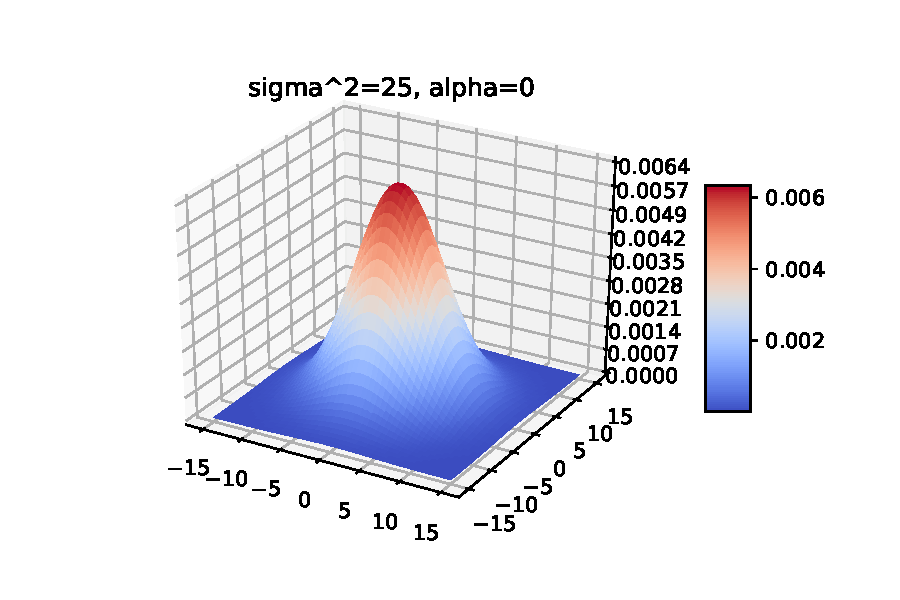
\includegraphics[width=0.5\textwidth]{images/plot-5-0-side.pdf} 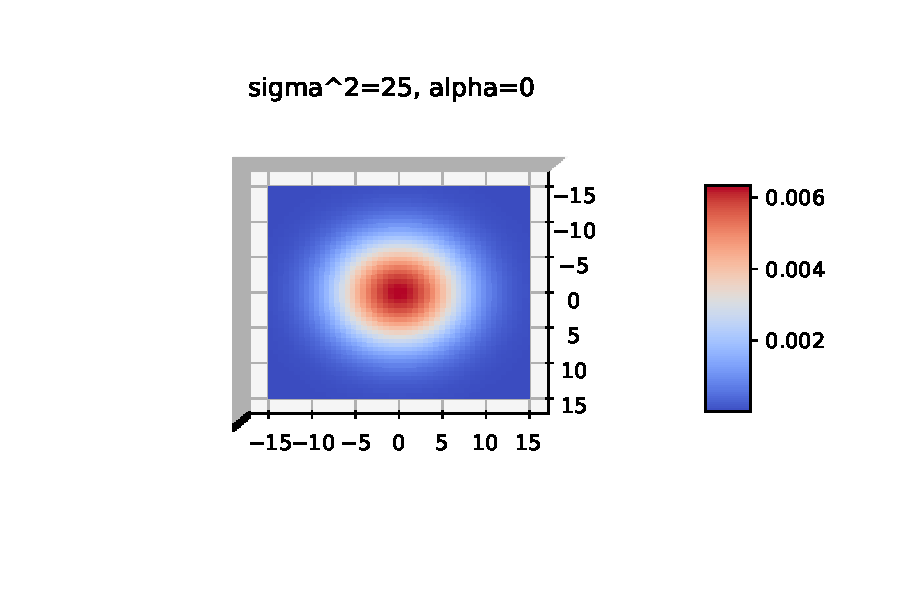
\includegraphics[width=0.5\textwidth]{images/plot-5-0-top.pdf}\\
 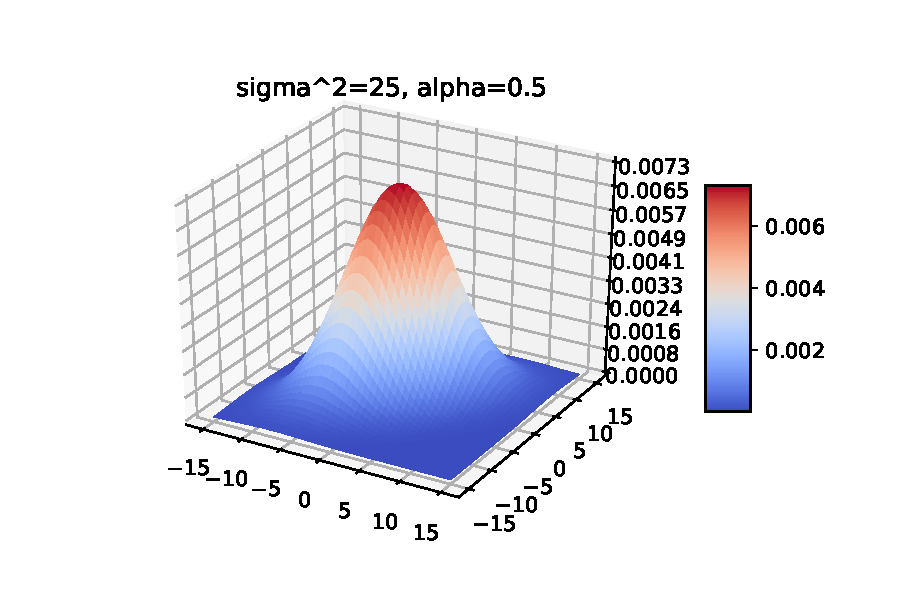
\includegraphics[width=0.5\textwidth]{images/plot-5-5-side.pdf} 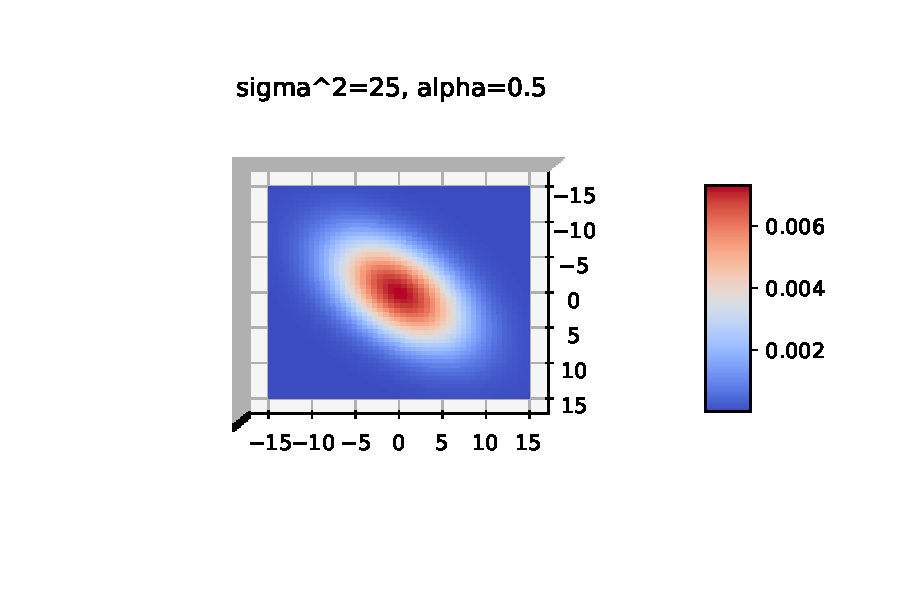
\includegraphics[width=0.5\textwidth]{images/plot-5-5-top.pdf}\\
 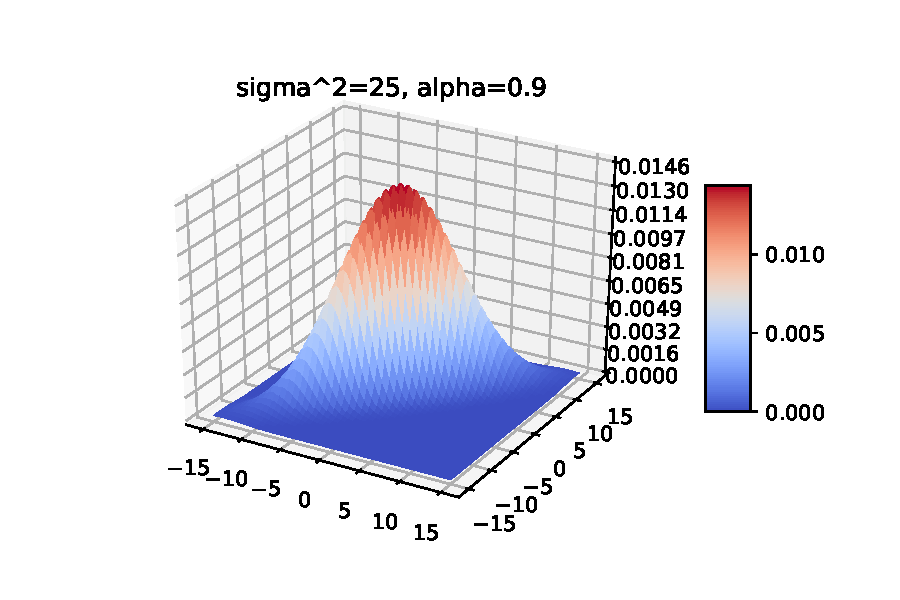
\includegraphics[width=0.5\textwidth]{images/plot-5-9-side.pdf} 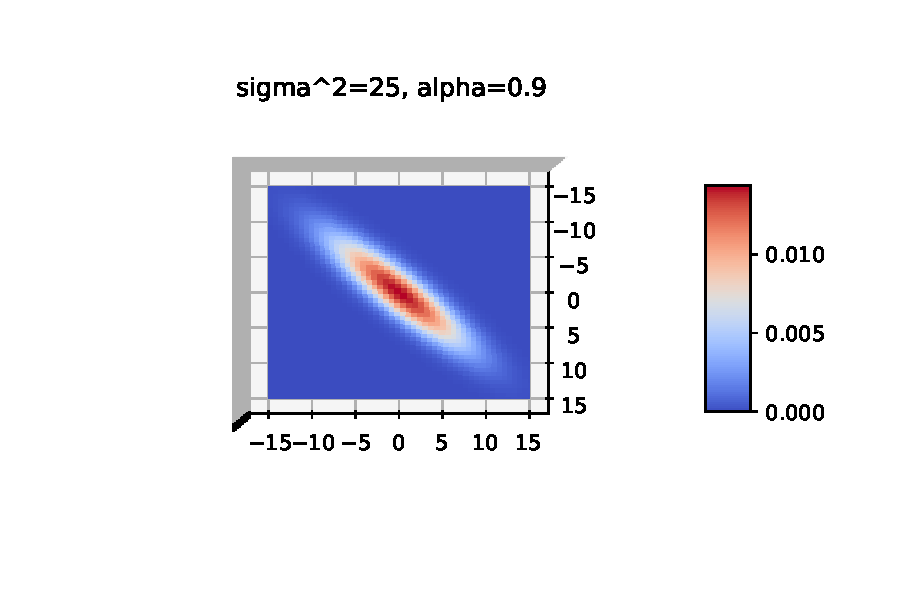
\includegraphics[width=0.5\textwidth]{images/plot-5-9-top.pdf}
 \caption{plots for $\sigma^2=25$}
\end{figure}
\begin{figure}
 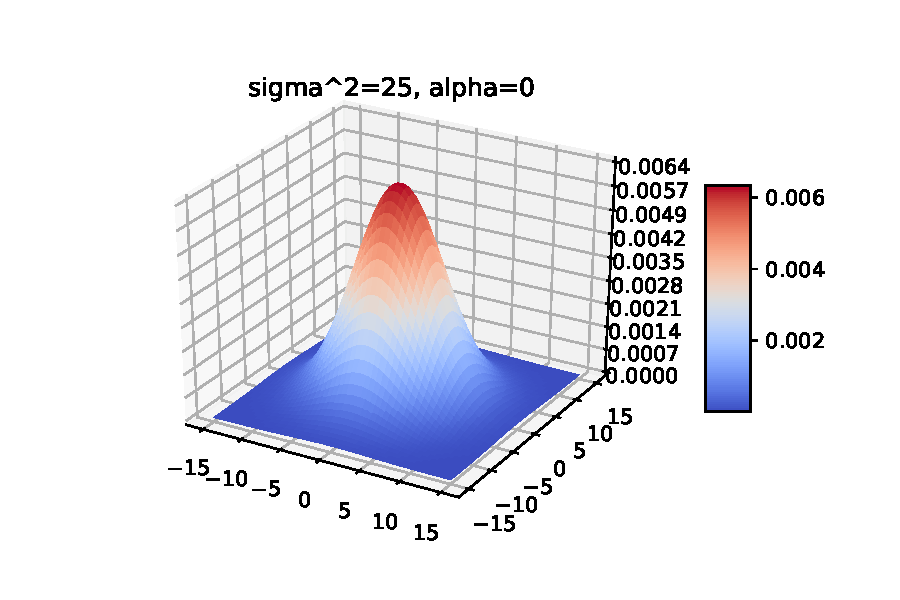
\includegraphics[width=0.5\textwidth]{images/plot-5-0-side.pdf} 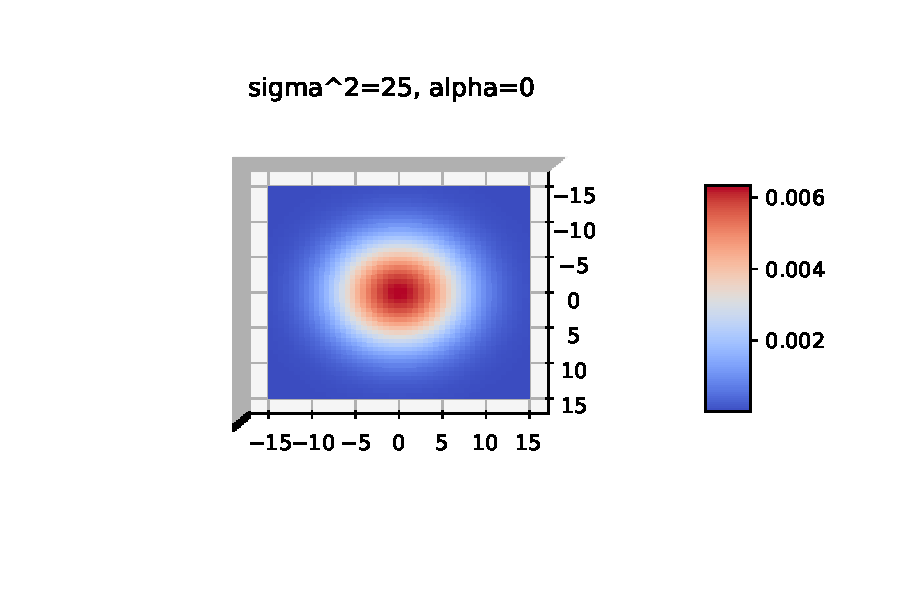
\includegraphics[width=0.5\textwidth]{images/plot-5-0-top.pdf}\\
 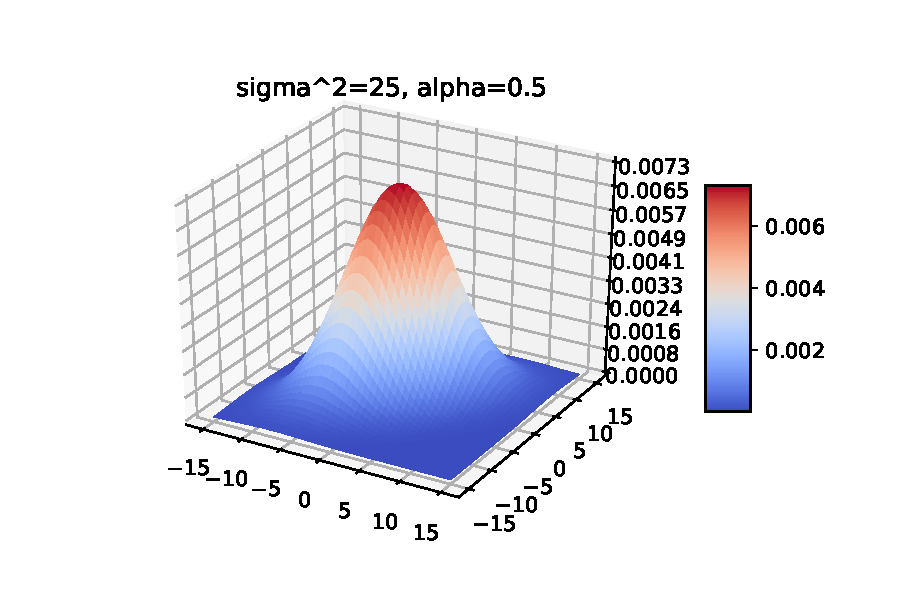
\includegraphics[width=0.5\textwidth]{images/plot-5-5-side.pdf} 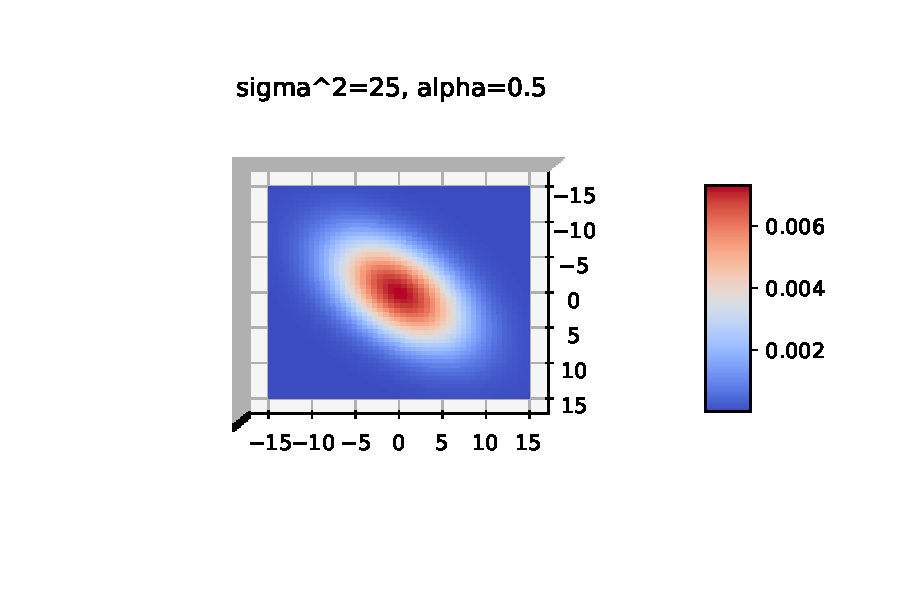
\includegraphics[width=0.5\textwidth]{images/plot-5-5-top.pdf}\\
 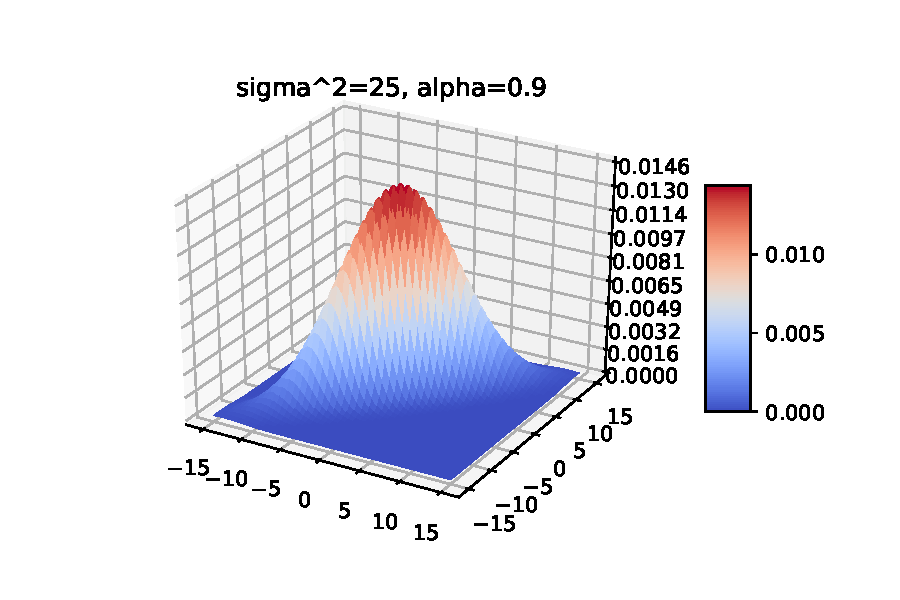
\includegraphics[width=0.5\textwidth]{images/plot-5-9-side.pdf} 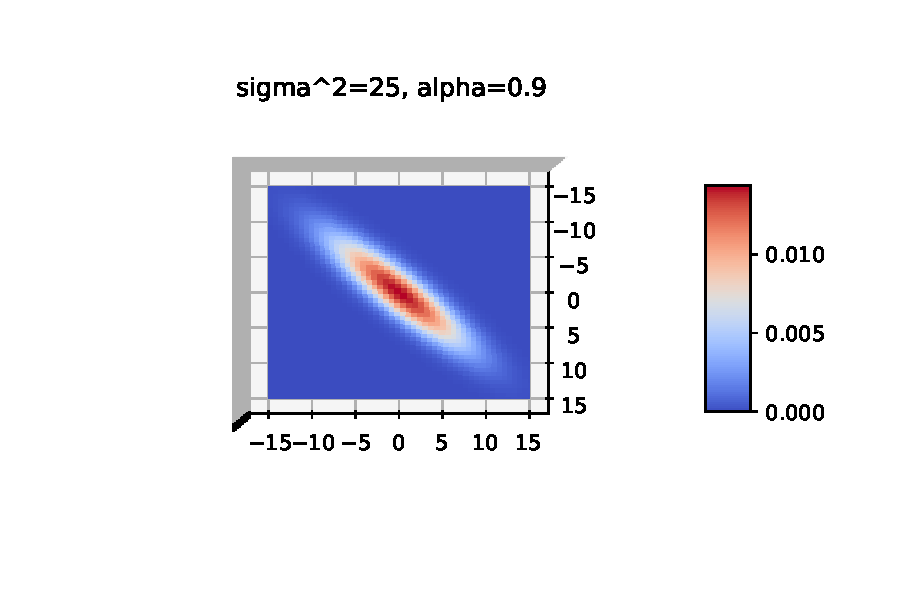
\includegraphics[width=0.5\textwidth]{images/plot-5-9-top.pdf}
 \caption{plots for $\sigma^2=100$}
\end{figure}
\par4. As described previously the marginal densities do not depend on $\alpha$. Also, because mean and variance for $X$ and $Y$ are equal, the plots for $X$ and $Y$ look the same for given $\sigma^2$. The plots are shown in figure 4.
\begin{figure}
 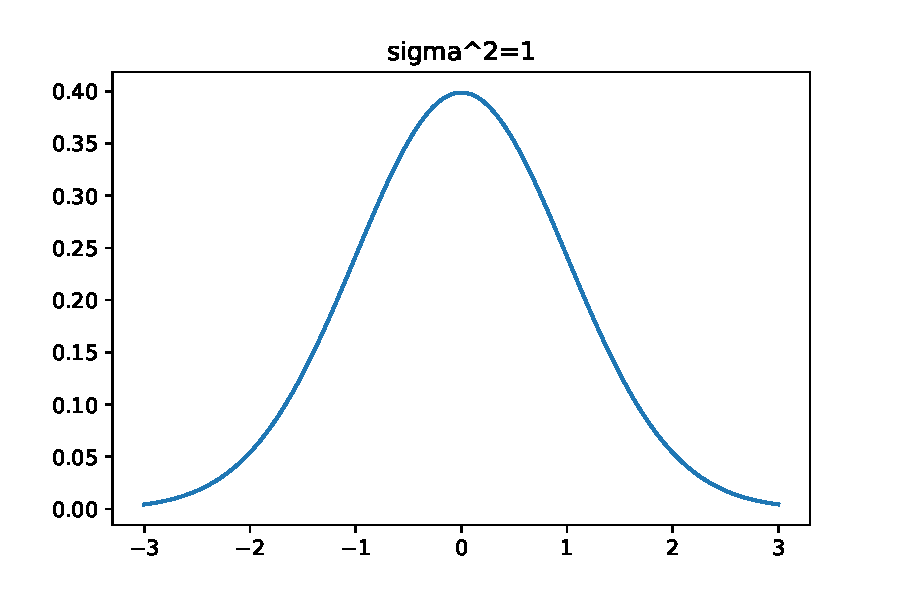
\includegraphics[width=0.3\textwidth]{images/plot-x-1.pdf}
 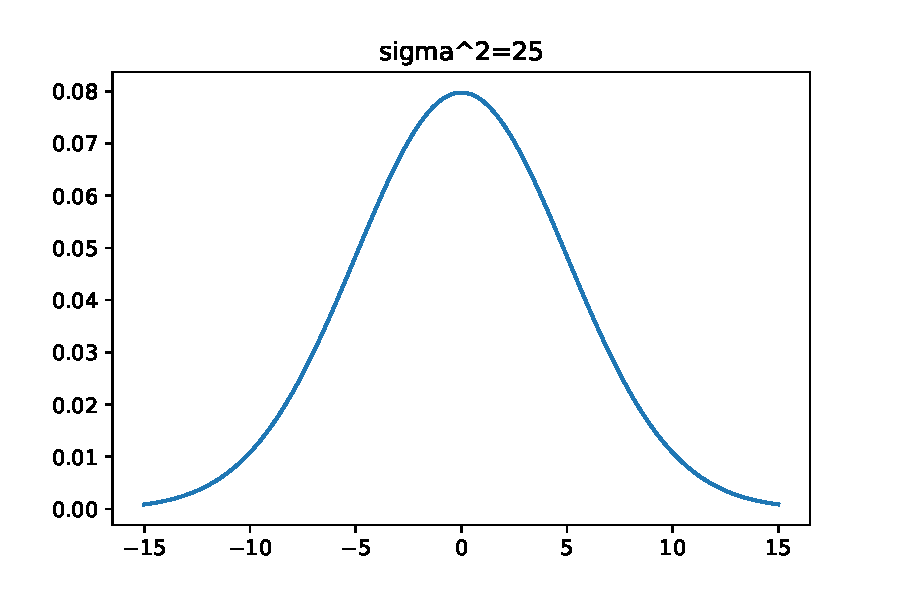
\includegraphics[width=0.3\textwidth]{images/plot-x-5.pdf}
 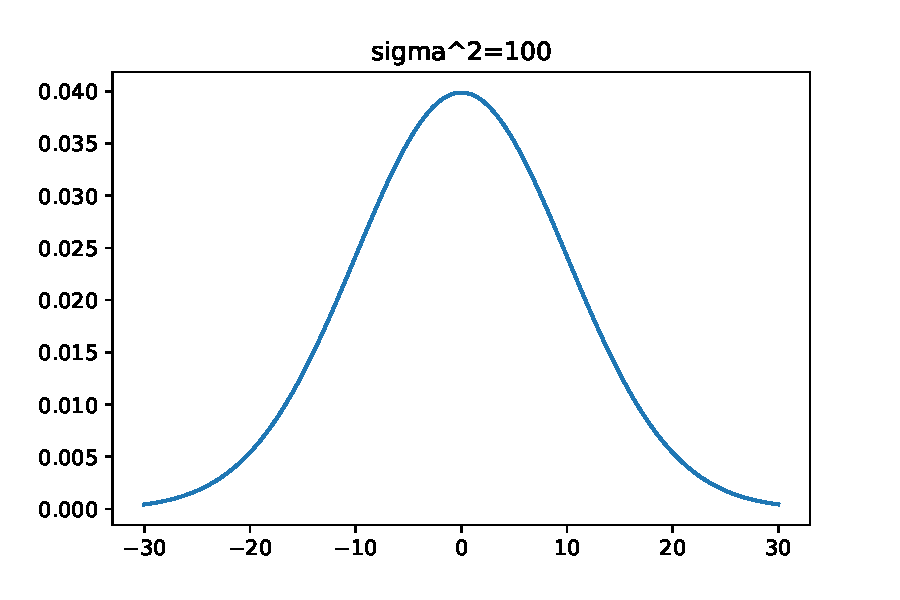
\includegraphics[width=0.3\textwidth]{images/plot-x-10.pdf}
 \caption{marginal densities of $X$ and $Y$}
\end{figure}
\end{solution}

\newpage
\begin{nexercise}{Empirical Risk Minimization}
\end{nexercise}
\begin{solution}
 1. We have
 \begin{equation*}
  R(y)=\int\int (y(x)-t)^2 p_{X,T}(x,t) dtdx=\int\int (y(x)-\E(T|Xx+\E(T|x)-t)^2 p_{X,T}(x,t) dt dx
 \end{equation*}
\begin{align*}
 =\int\int (y(x)-\E(T|x))^2 p_{X,T}(x,t)dtdx+2\int\int (y(x)-\E(T|x))(\E(T|x)-t)p_{X,T}(x,t) dtdx \\+\int\int (\E(T|x)-t)^2 p_{X,T}(x,t)dtdx
\end{align*}
\begin{align*}
 =\int\int (y(x)-\E(T|x))^2 p_{X,T}(x,t)dtdx+2\int (y(x)-\E(T|x))\underbrace{\int (\E(T|x)-t)\frac{p_{X,T}(x,t)}{p_X(x)} dt}_{=0}p_X(x)dx \\+\int\underbrace{\int (\E(T|x)-t)^2 \frac{p_{X,T}(x,t)}{p_X(x)}dt}_{=\var(T|x)}p_X(x)dx.
\end{align*}
\begin{equation}\label{eq1}
 =\int (y(x)-\E(T|x))^2 p_X(x)dx+0+\int \var(T|x) p_X(x)dx
\end{equation}
The choice of $y$ has no impact on the second integral, so minimizing this expression is equivalent to minimizing the first integral. The integrand is non-negative, so the integral can be at least 0. This is the case iff $y(x)=\E(T|x)$ almost everywhere, so the choice $y(x)=\E(T|x)$ minimizes the expected loss. In our example we have
\begin{equation*}
 \E(T|x)=\int t p_T(t|x)=\int (\sin(x)+s)\frac{1}{\sqrt{2\pi\sigma^2}}\exp(-\frac{s^2}{2\sigma^2})ds=\sin(x),
\end{equation*}
so $y^*(x)=\sin(x)$.\\
\par2. To find the minimizer $w^*$, consider
\begin{equation*}
 ||\Phi w-t||^2=(\Phi w-t)^T(\Phi w-t)=(\Phi w)^T(\Phi w)-(\Phi w)^Tt -\underbrace{t^T(\Phi w)}_{=(\Phi w)^Tt\text{ (scalar)}}+t^Tt
\end{equation*}
\begin{equation*}
 =(\Phi w-t)^T(\Phi w-t)=w^T\Phi^T\Phi w-2(\Phi w)^Tt +t^Tt
\end{equation*}
\begin{equation*}
 \Rightarrow \frac{\partial}{\partial w_i} ||\Phi w-t||^2= \frac{1}{N}\left( 2\underbrace{\Phi_{(i)}^T}_{\text{i-th line of $\Phi$}}\Phi w-2\Phi_{(i)}^Tt\right)\stackrel{!}{=}0 ~ \forall i=1,...N
\end{equation*}
\begin{equation*}
 \Rightarrow \nabla_w ||\Phi w-t||^2= \frac{1}{N}\left( 2\Phi^T\Phi w -2\Phi^Tt\right)\stackrel{!}{=}0\Leftrightarrow 2 \Phi^T\Phi w=2\Phi^Tt \Leftrightarrow w=(\Phi^T\Phi)^{-1}\Phi^T t.
\end{equation*}
The matrix $\Phi^T\Phi$ is invertible, if all $x_i$ are distinct, because in this case $\Phi$ has rank $p$, as its first $p$ rows from a Vandermonde matrix. Moreover
\begin{equation*}
 \frac{\partial^2}{\partial w_i \partial w_j} ||\Phi w-t||^2 =\frac{1}{N} 2\Phi_{(i)}^T\Phi_{(j)},
\end{equation*}
which is positive definite, as $\Phi$ has full rank, so the found point $w^*= (\Phi^T\Phi)^{-1}\Phi^T t$is indeed a minimum.\\
\begin{figure}
  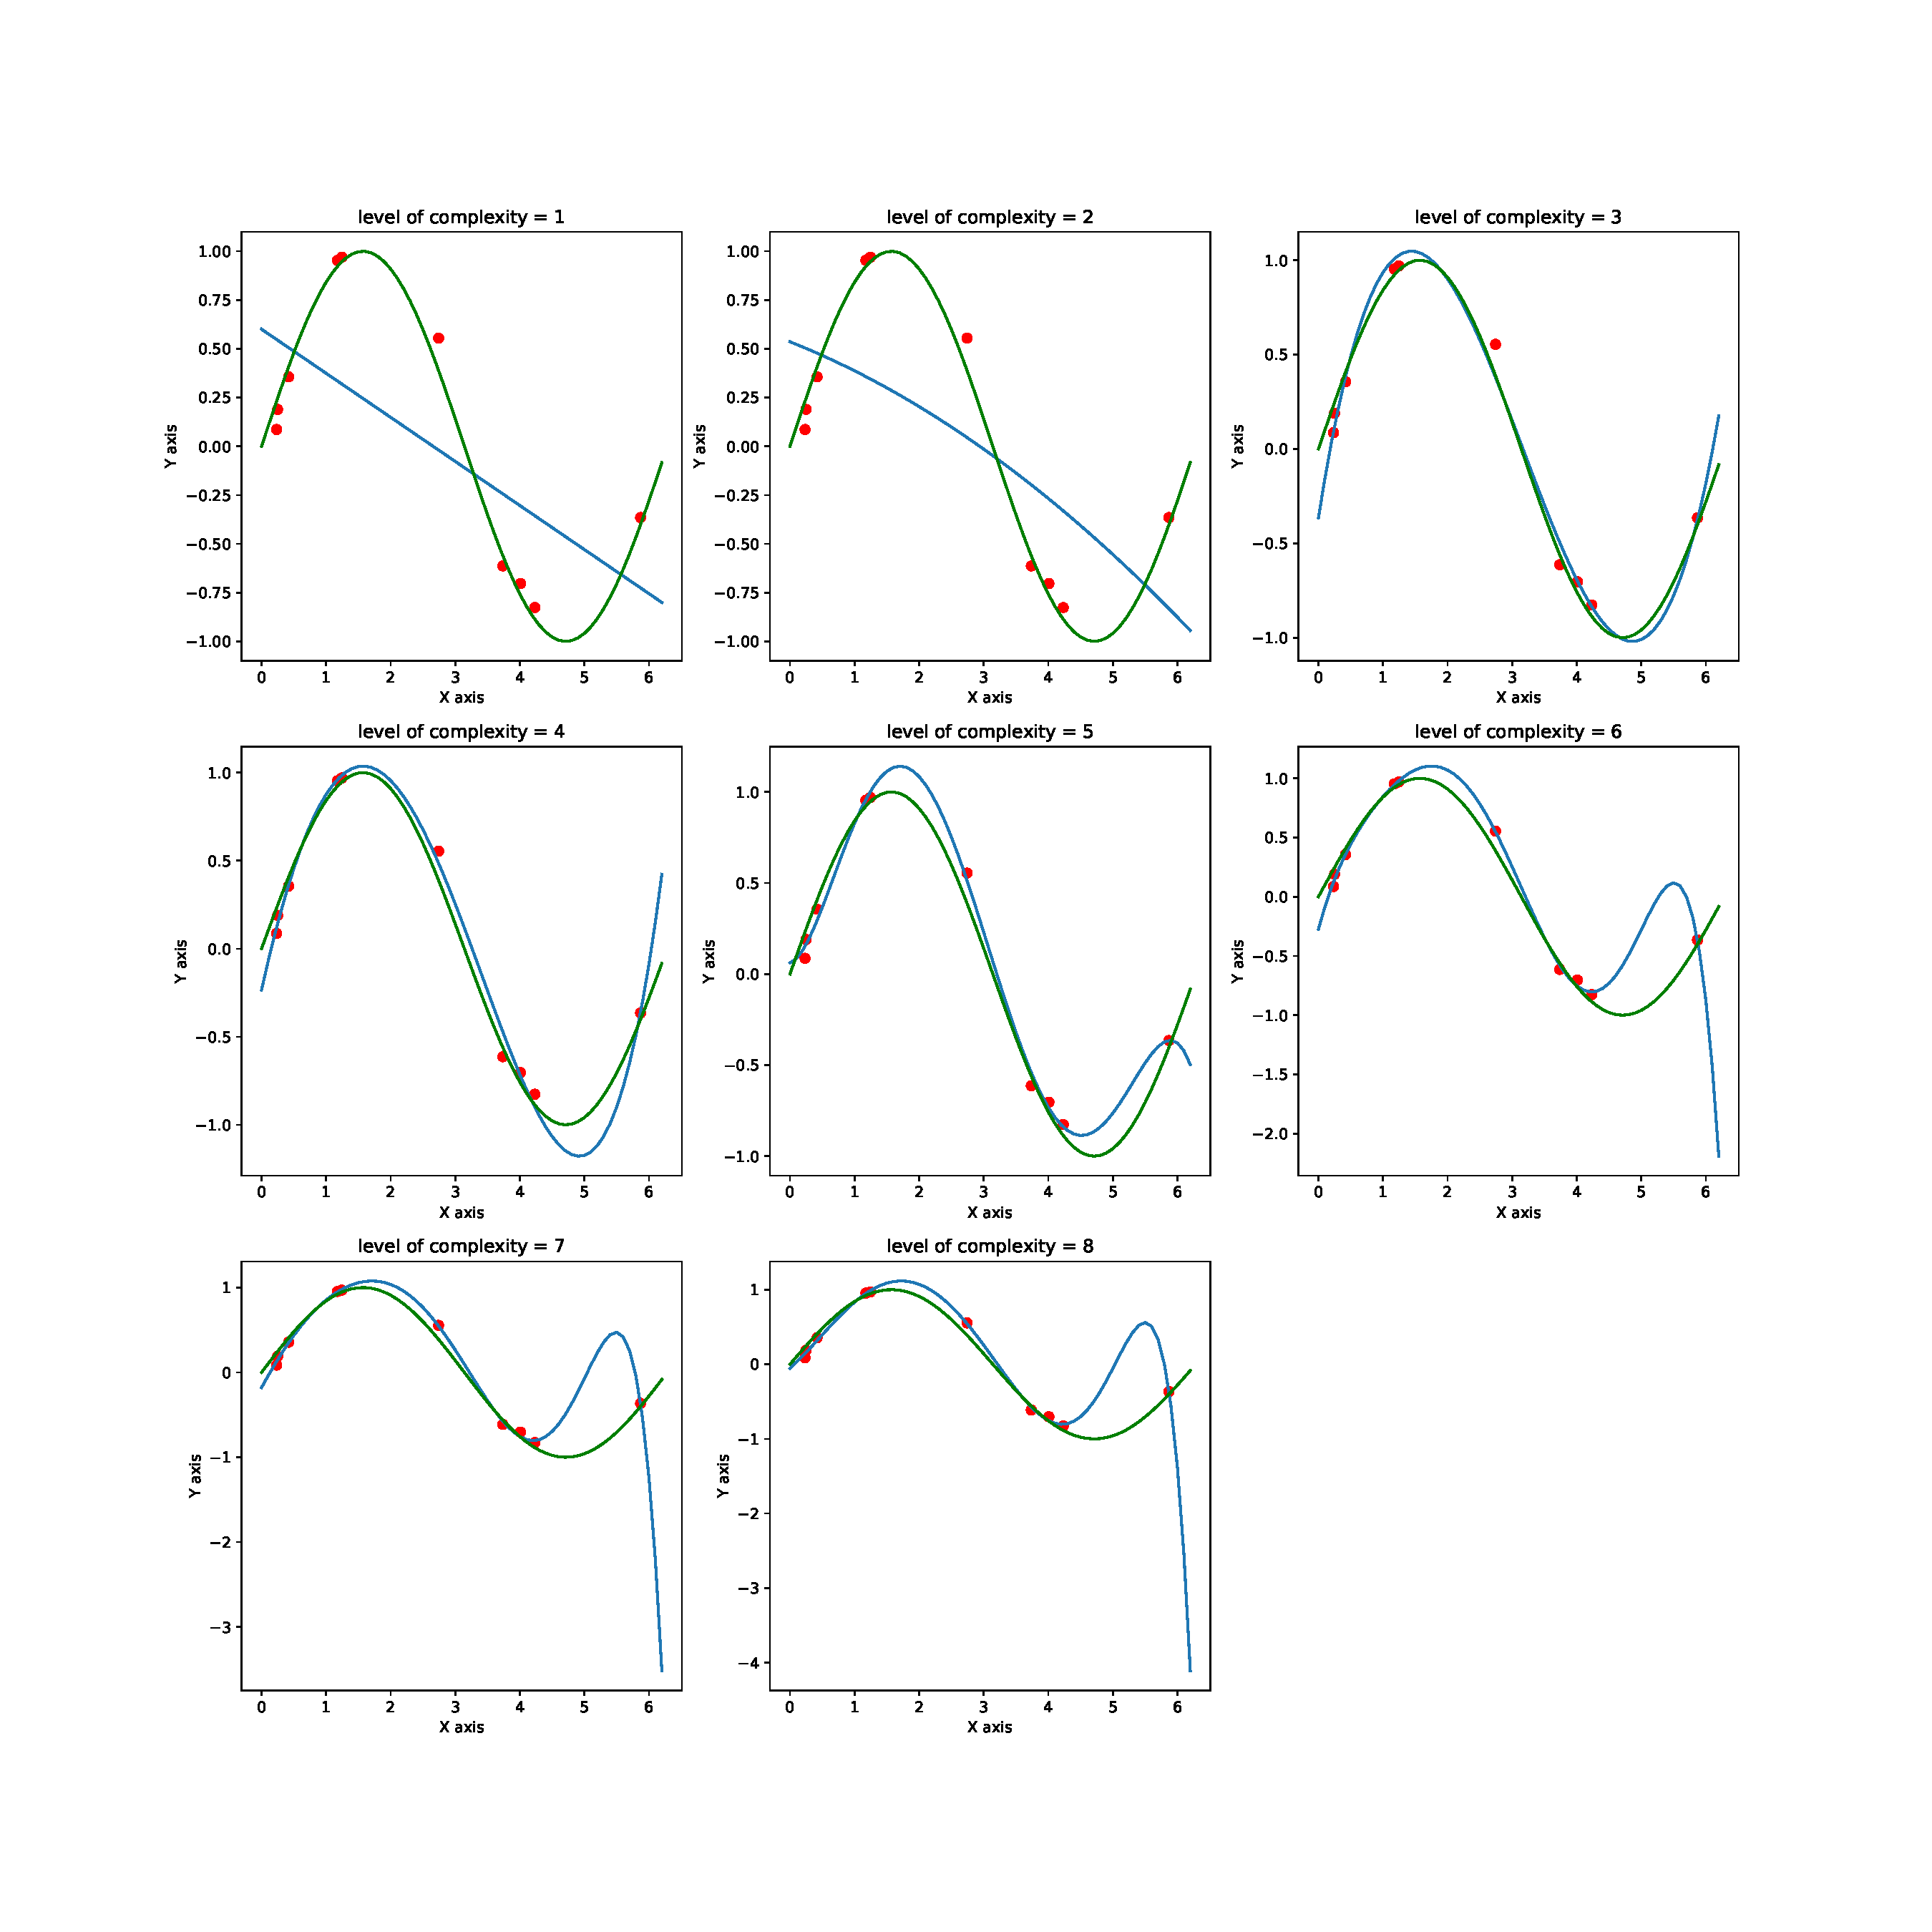
\includegraphics[width=\textwidth]{images/samples-10.pdf}
  \caption{regression functions for $N=10$ points}
  \label{samp10}
 \end{figure}
 \begin{figure}
  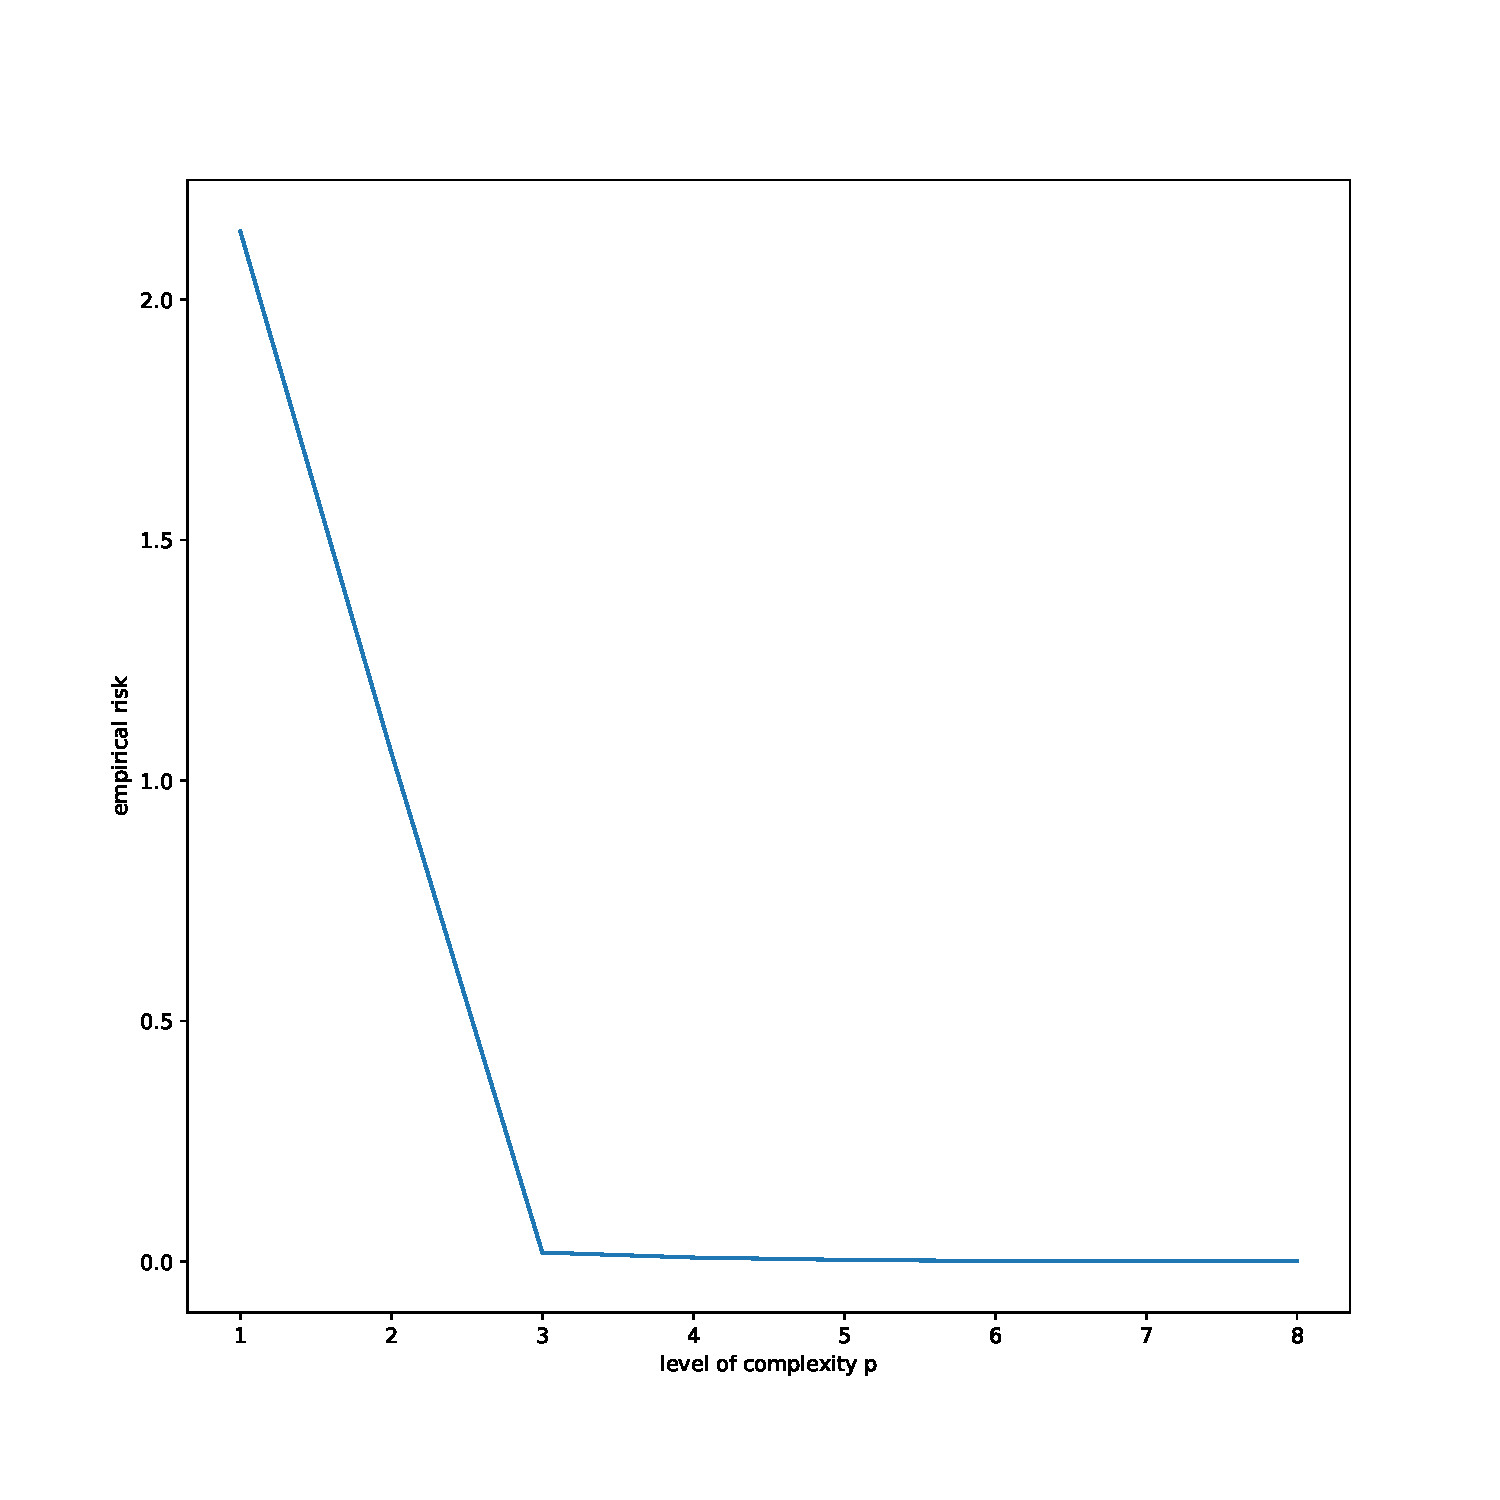
\includegraphics[width=0.4\textwidth]{images/empirical_risk-10.pdf}
  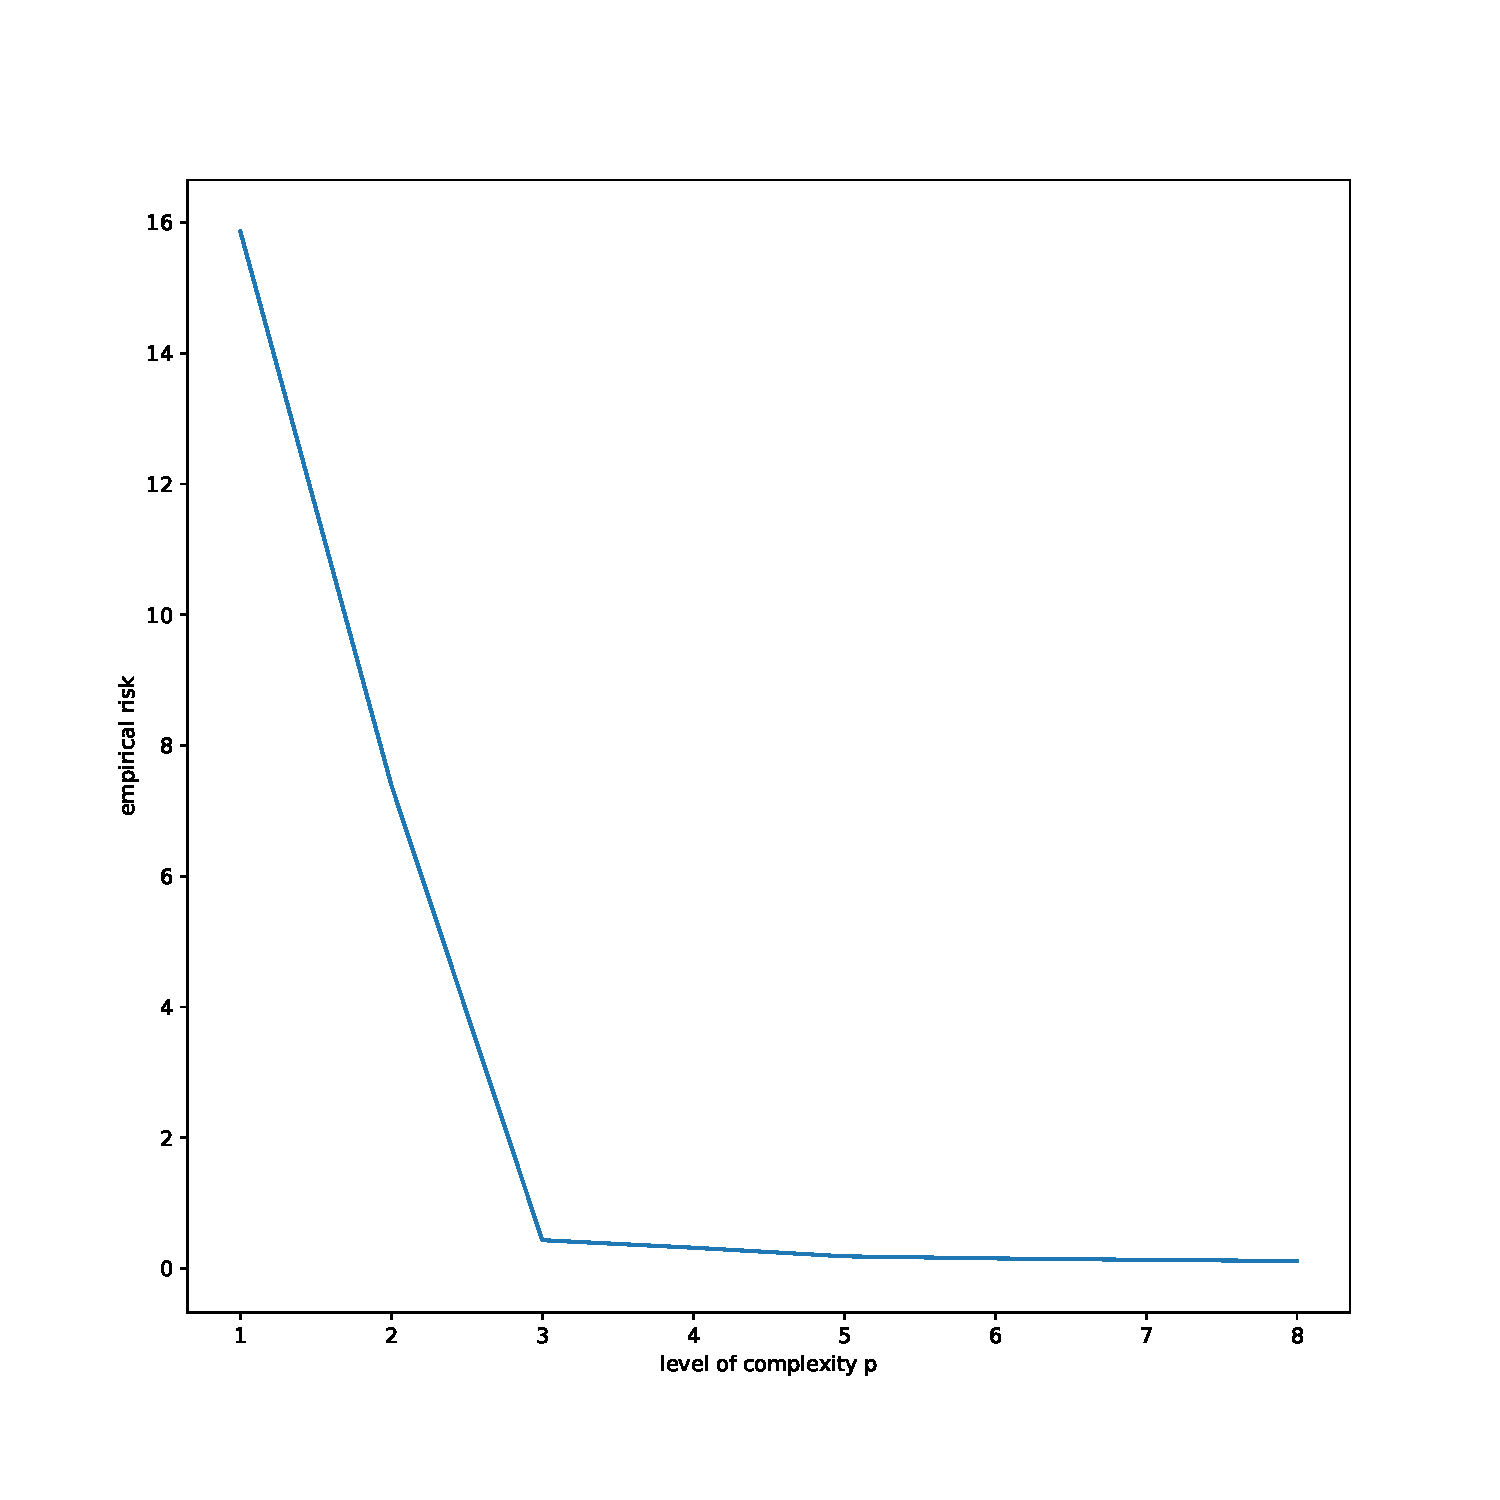
\includegraphics[width=0.4\textwidth]{images/empirical_risk-100.pdf}
  \caption{empirical risk for $N=10$ and $N=100$ points}
  \label{emr}
 \end{figure}
 \begin{figure}
  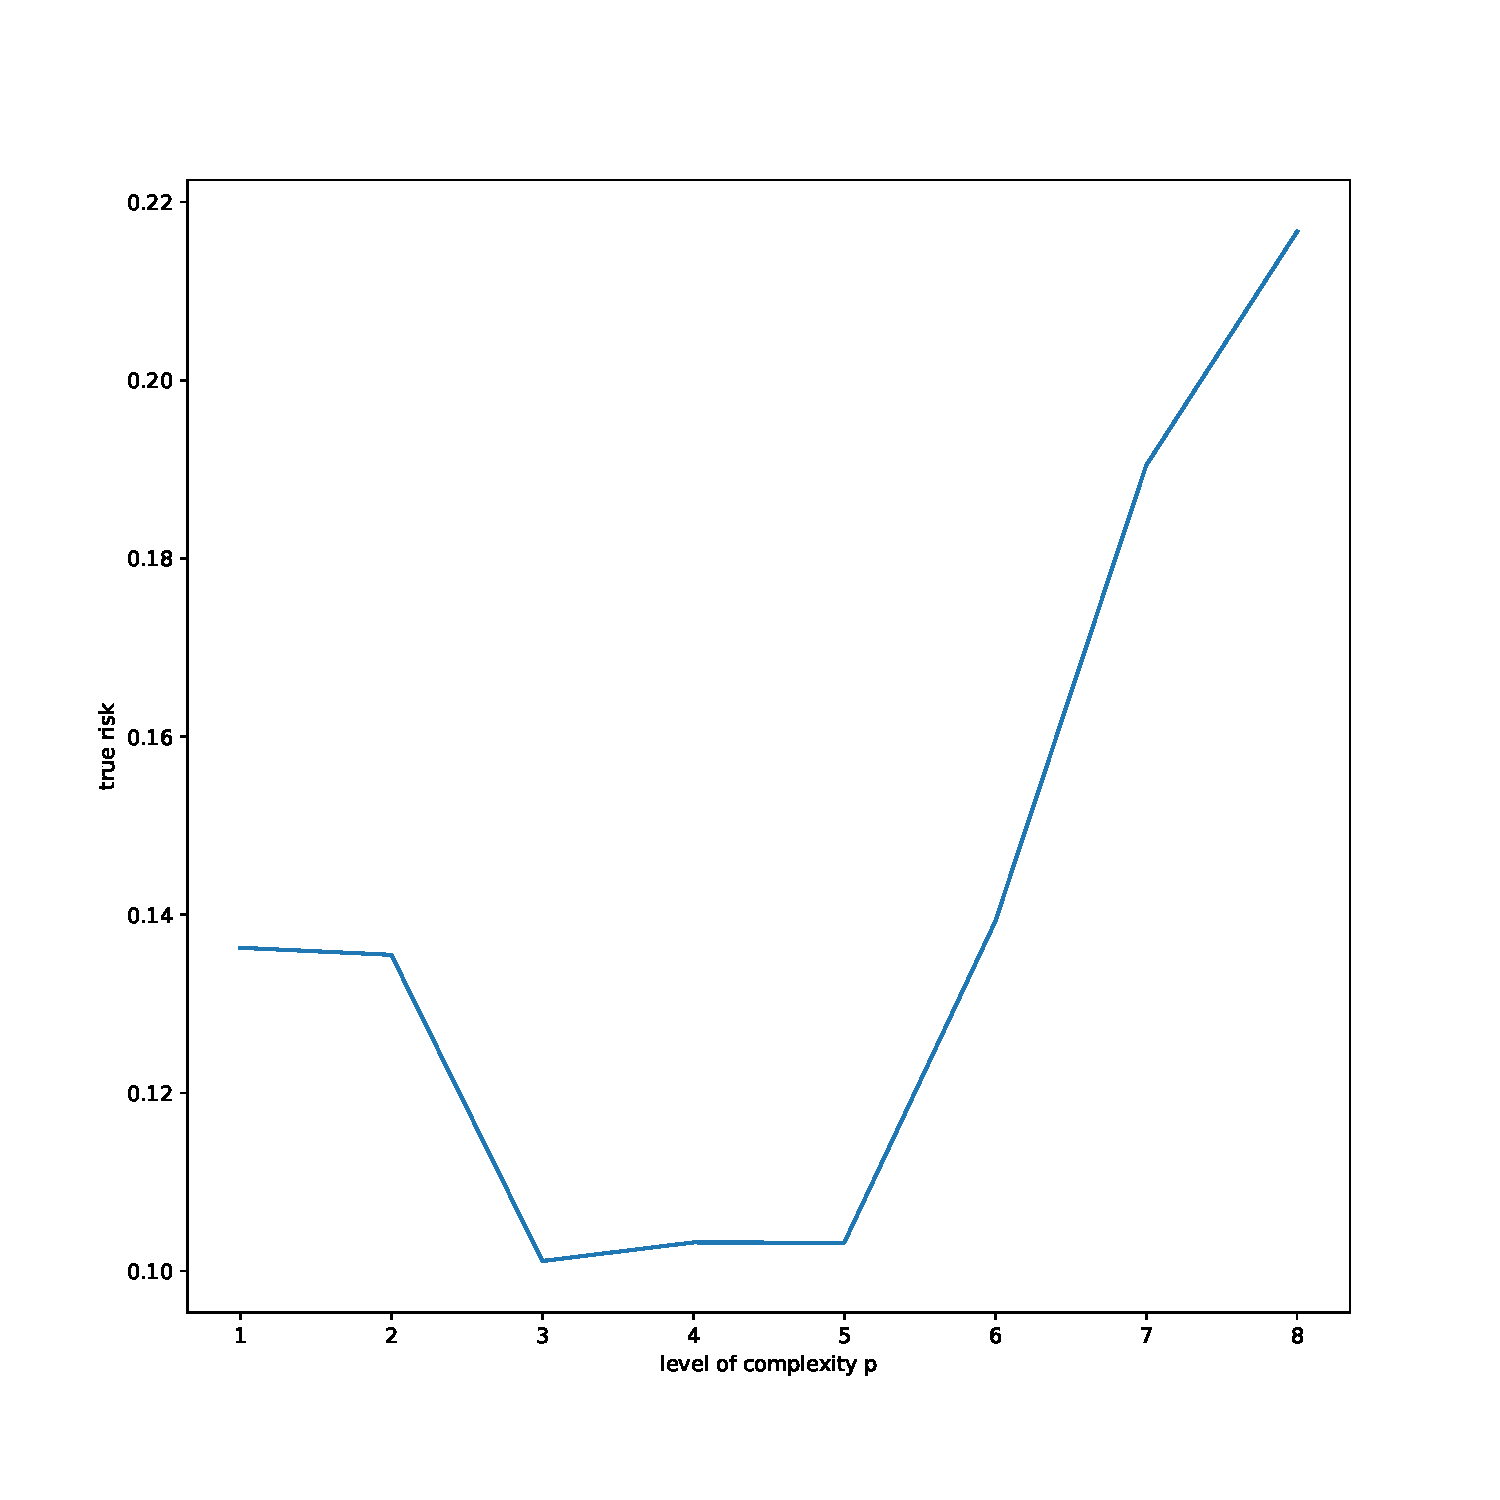
\includegraphics[width=0.4\textwidth]{images/true_risk-10.pdf}
  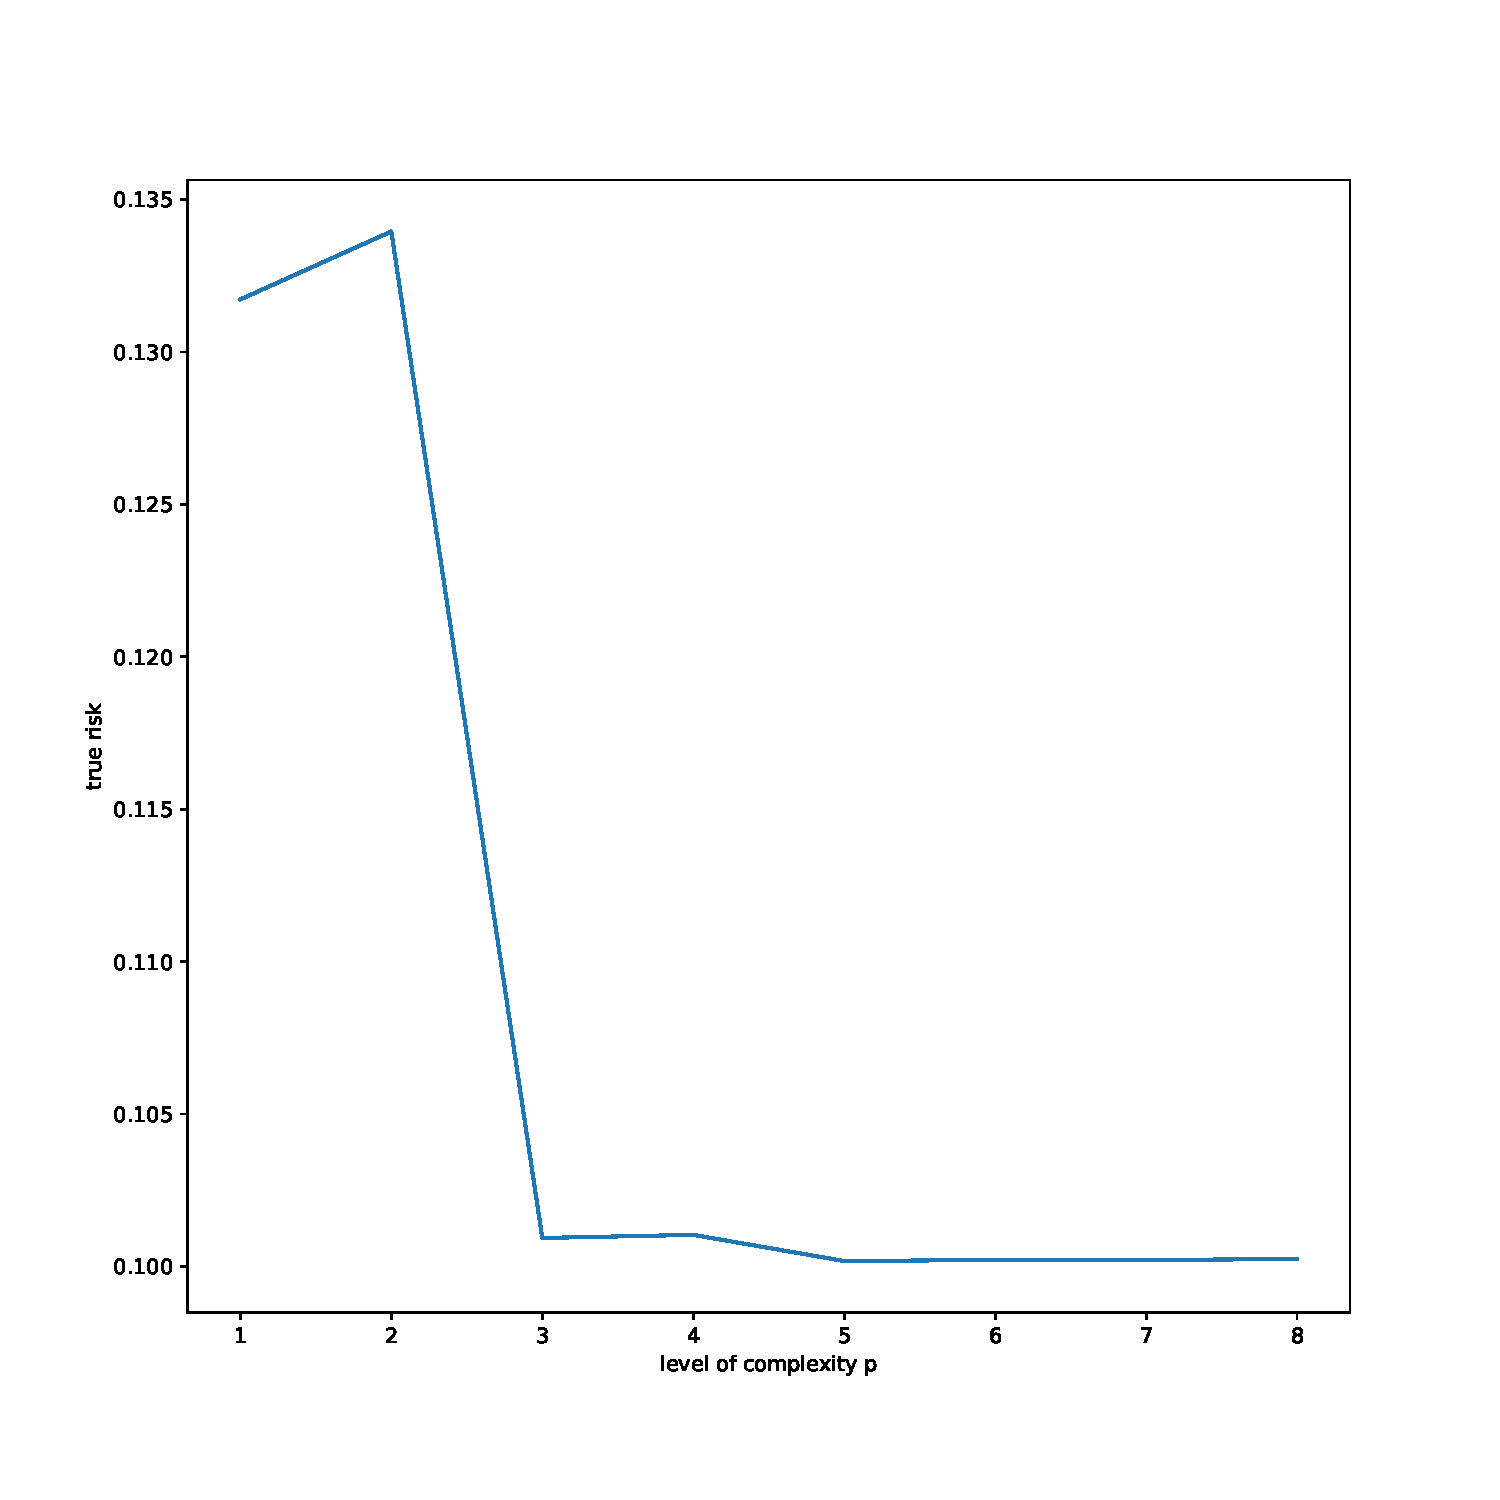
\includegraphics[width=0.4\textwidth]{images/true_risk-100.pdf}
  \caption{true risk for $N=10$ and $N=100$ points}
  \label{tr}
 \end{figure}
 \begin{figure}
  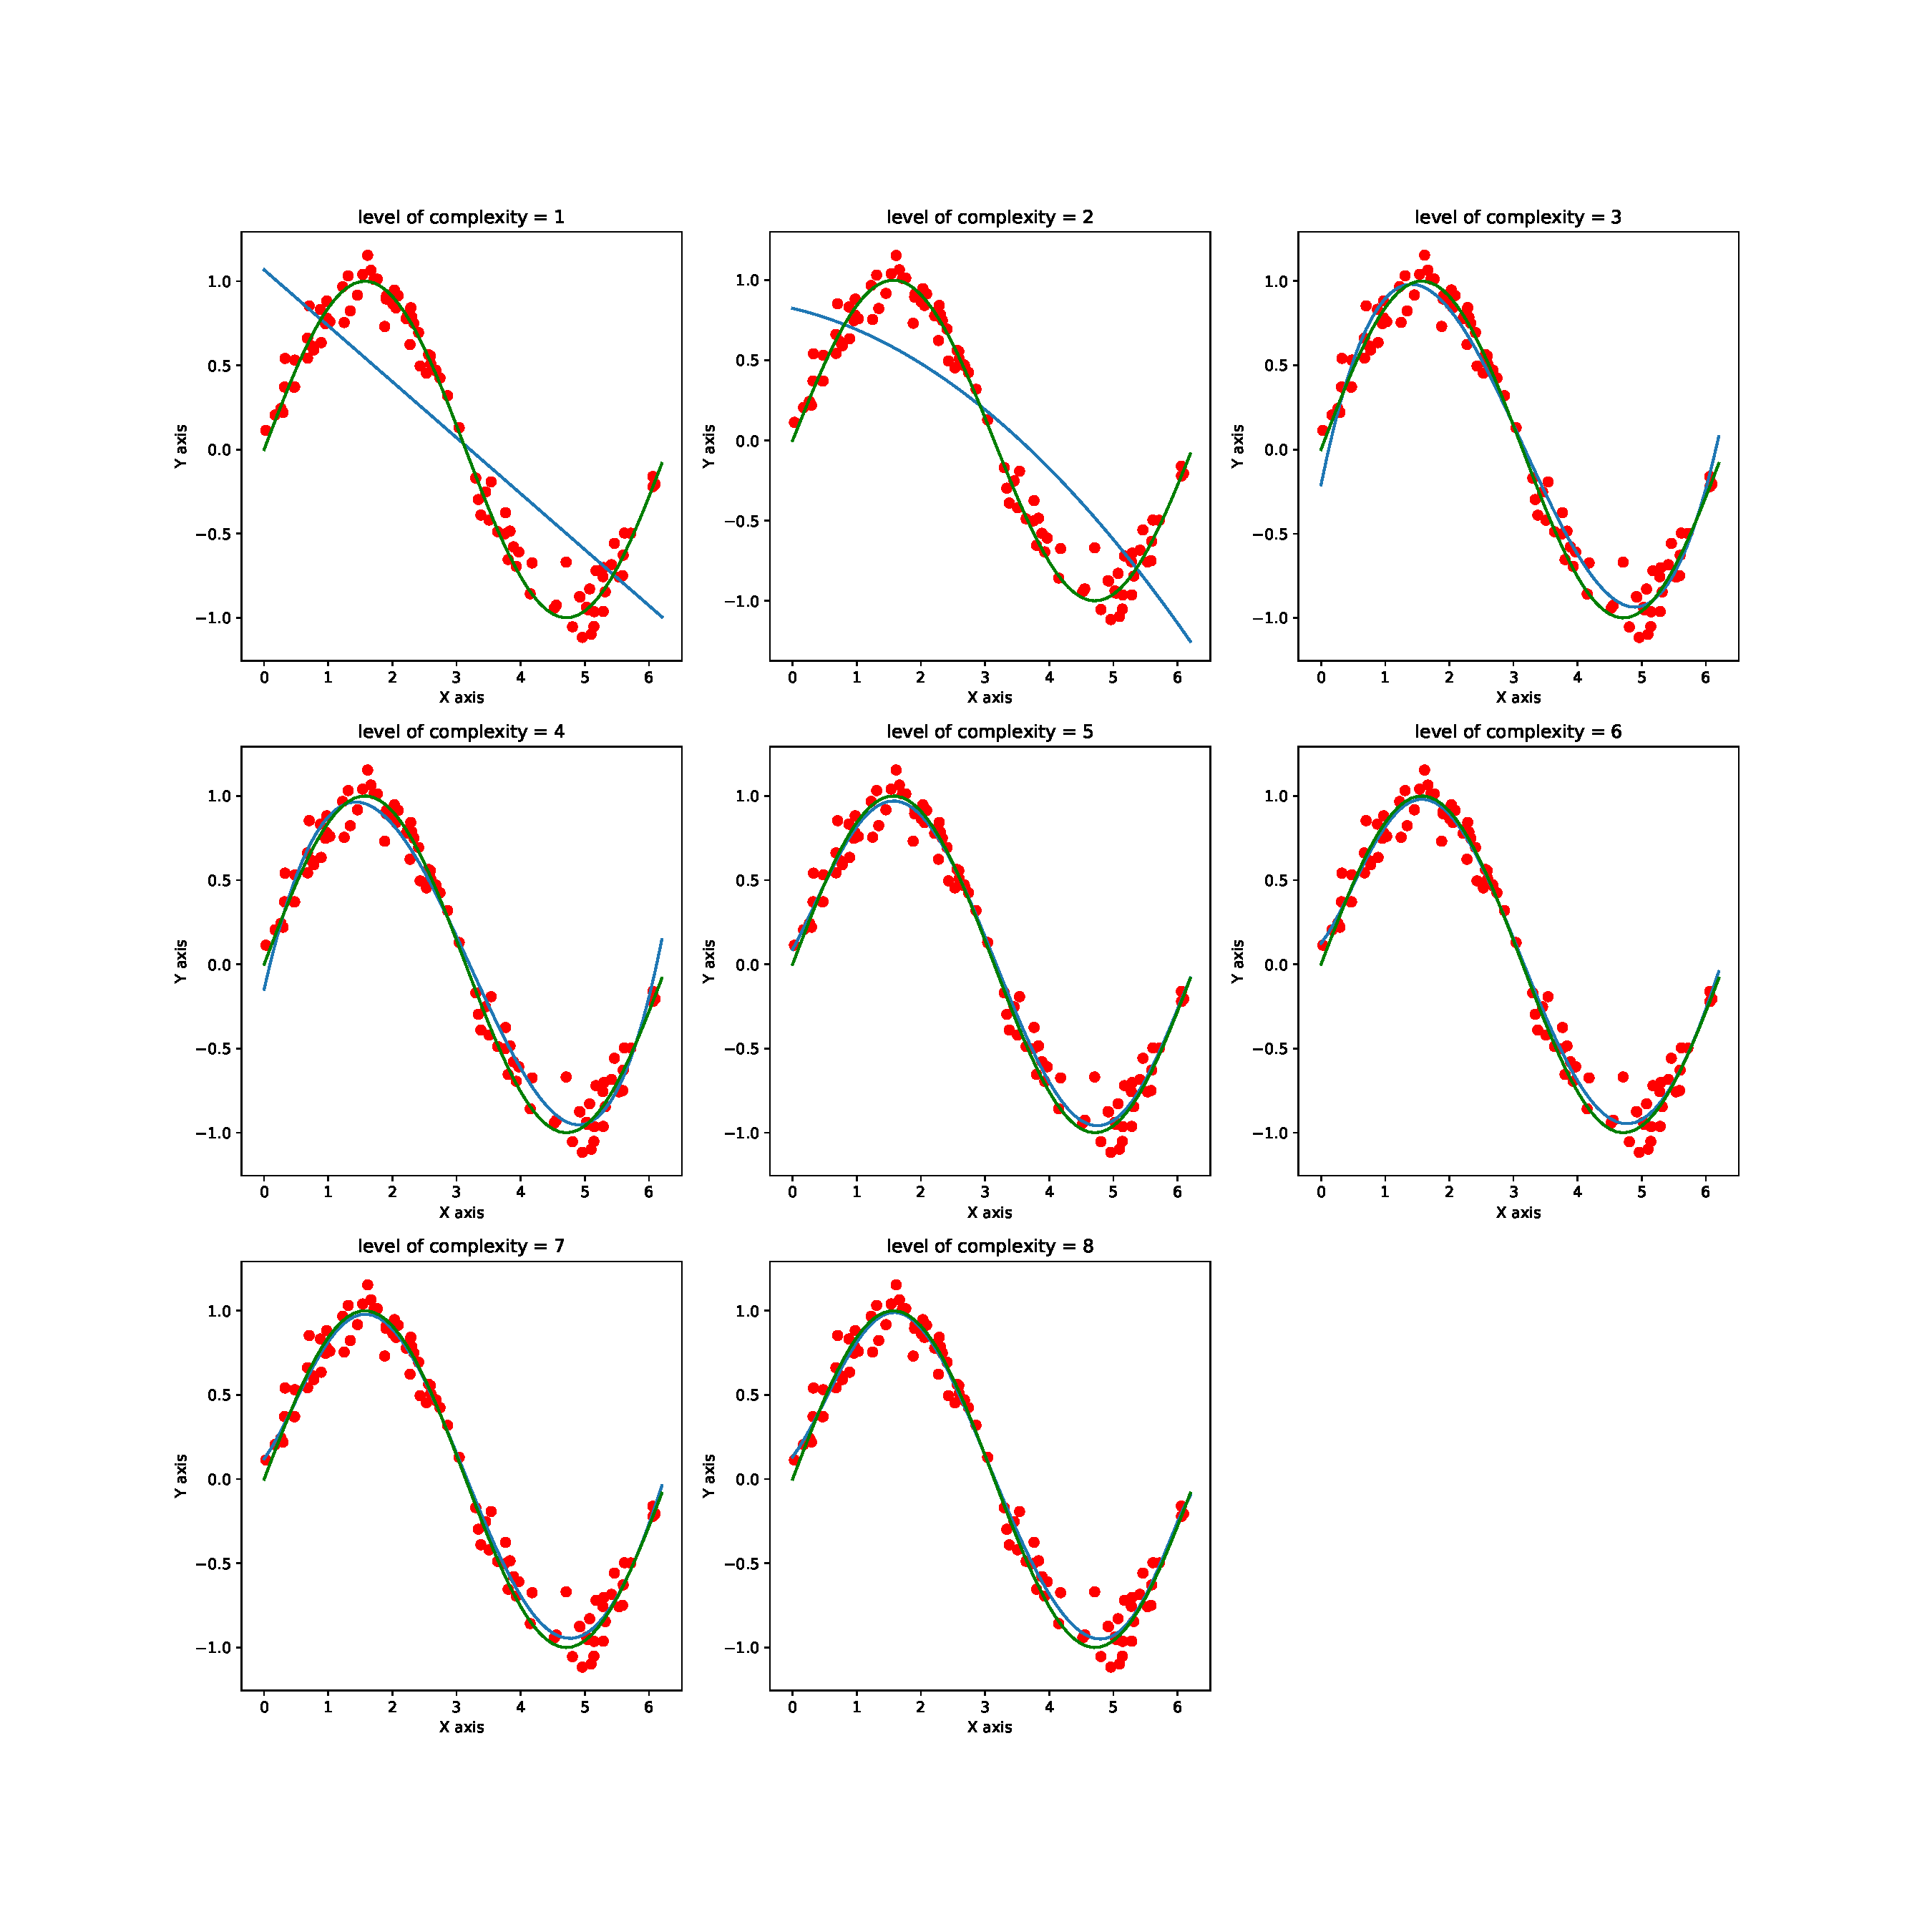
\includegraphics[width=\textwidth]{images/samples-100.pdf}
  \caption{regression functions for $N=100$ points}
  \label{samp100}
 \end{figure}
\par3.-6. The plots for $N=10$ are shown in figure \ref{samp10}, the empirical risks in figure \ref{emr}. To compute the true risk, we use the decomposition of equation \ref{eq1}. We approximate the first integral by uniform sampling on $\lbrack 0, 2\pi\rbrack$. To evaluate the second, note, that the conditional density $p_T(t|x)$ is the normal density of $\eta$ (constant in $x$), so
\begin{equation*}
 \var(T|x)=\int (t-\E(T|x))^2 p_T(t|x)dt=\int \eta^2 p_N(\eta) d\eta=\var(\eta)=\sigma^2
\end{equation*}
and therefore
\begin{equation*}
 \int \var(T|x) p_X(x)dx=\sigma^2.
\end{equation*}
The plots of the true risks are given in figure \ref{tr}. For both $x$-datasets the empirical risk decreases monotonously in the complexity level. This makes sense, because with a hight complexity level there are more degrees of freedom, so the polynomial can be chosen such that the curve is closer to the chosen points. For $N=10$ the true risk is minimal for $p=3$, for higher complexity the risk is higher again. The reason for this is overfitting. We have almost as many degrees of freedom as we have points to fit. The polynomial is calculated to fit the 10 chosen points as well as possible, but this comes at the cost of (almost) all other points on the curve. This is also visible in the plots, the regression function is very close to the red points, but for points, that lie a bit further away from the sample points, the curve isn't close at all. The quality of the regression here depends much on how the 10 sample points are distributed in the interval $\lbrack0,2\pi\rbrack$. For different sample points (in different tests) the minimum was reached at a different complexity level, sometimes even at p=8.\\
For $N=100$ the true risk decreases monotonously with a higher complexity level. In this case no overfitting occurs, because even for $p=8$ there are many more points to be fitted than degrees of freedom. This is also visible in the regression plots for $N=100$ (figure \ref{samp100}). The larger the complexity level is, the better the regression function fits the sample points.
\end{solution}

\newpage
\begin{nexercise}{MNIST - Bayesian Denoising}
\end{nexercise}
\begin{solution}
 We assume, that $p(Y=y_n)=p(Y=y_1)=c$ for all $n=1,...,N$, but no uniform distribution on $\lbrack 0,1\rbrack^D$, because that would mean $p(Y=y_n)=0~\forall n=1,...,N$, which would lead to troubles in the definition of the conditional probability in the original sense.
 \par1. We have
 \begin{equation*}
  \frac{\sum_{n=1}^N y_np(X=x|Y=y_n)}{\sum_{n=1}^N p(X=x|Y=y_n)}=\frac{\sum_{n=1}^N y_np(X=x,Y=y_n)/p(Y=y_n)}{\sum_{n=1}^N p(X=x,Y=y_n)/p(Y=y_n)}=\frac{\frac{1}{c}\sum_{n=1}^N y_np(X=x,Y=y_n)}{\frac{1}{c}\sum_{n=1}^N p(X=x,Y=y_n)}
 \end{equation*}
\begin{equation*}
 =\frac{\sum_{n=1}^N y_np(X=x,Y=y_n)}{\sum_{n=1}^N p(X=x,Y=y_n)}=\frac{\sum_{n=1}^N y_np(X=x,Y=y_n)}{p(X=x)}
 \end{equation*}
 \begin{equation*}
 =\sum_{n=1}^N y_n p(Y=y_n|X=x)=\E_Y(Y|X=x)=\hat{y}_{CM}(x)
\end{equation*}
\par2. We have (because $\frac{c}{p(X=x)}>0$)
\begin{equation*}
 \arg \max_{y_n} p(X=x|Y=y_n) = \arg \max_{y_n} \frac{c}{p(X=x)}p(X=x|Y=y_n)=\arg \max_{y_n} \frac{c}{p(X=x)}\frac{p(X=x,Y=y_n)}{c}
\end{equation*}
\begin{equation*}
 =\arg \max_{y_n} \frac{p(X=x,Y=y_n)}{p(X=x)}=\hat{y}_{MAP}(x)
\end{equation*}
\par3.-11. The original images are shown in figure \ref{orgs}, figures \ref{s25}-\ref{s1} show the noisy images and the ones denoised with conditional mean and denoised with MAP (in this order).\\
As one would expect, a higher variance results in more difficult to read noisy images. This also increases the number of wrongly denoised images.\\
The images denoised with with the CM tend to be more blury then the ones denoised with MAP (especially for strong noise). This comes from the fact, that MAP just selects an already existing image, so the results of MAP can only be as blurry as the blurriest given image. The results of CM are weighted superpositions of the images in $Y_{test}$, this leads to the not so clear images. This has the disadvantage that the results themselves might be difficult to read, but the fact that noisy images, for which it is very unclear, from which original number they come, result in images that look similar to more than one image in $Y_{test}$ could also be seen as an advantage, depending on the application, because the uncertainty is visible in the result. If the MAP denoising selects one image it is impossible too see, whether the decision was very clear or there was a second image in $Y_{test}$ (possibly reflecting a different number) that was almost equally likely as the chosen one. The results from the CM can be made less blurry by iterating, i.e., calculating the conditional mean w.r.t. the conditional mean of the original image and so on.\\
The CM approach seems to do more mistakes for high variance than the MAP approach.


\begin{figure}
\begin{center}
 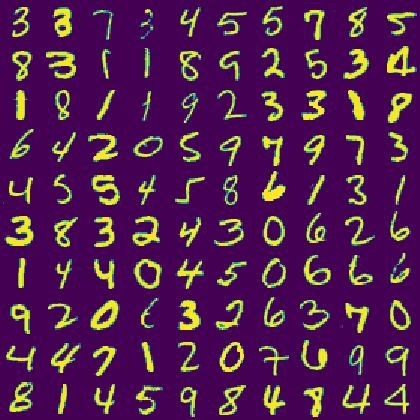
\includegraphics[width=0.5\textwidth]{images/originals.pdf}
 \end{center}
 \caption{original images}
 \label{orgs}
\end{figure}

\begin{figure}
 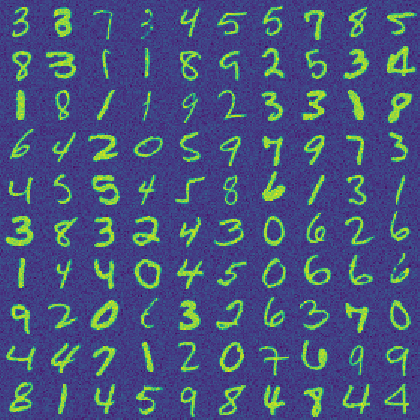
\includegraphics[width=0.3\textwidth]{images/noisy-25.pdf}
 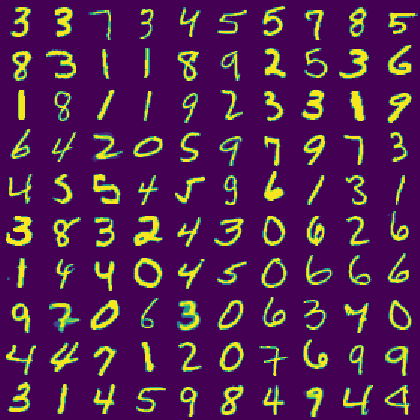
\includegraphics[width=0.3\textwidth]{images/denoised-25-mean.pdf}
 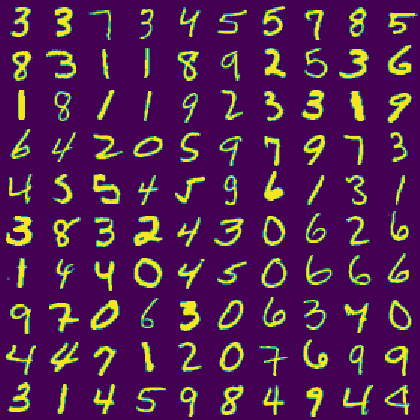
\includegraphics[width=0.3\textwidth]{images/denoised-25-map.pdf}
 \caption{$\sigma$=0.25}
 \label{s25}
\end{figure}

\begin{figure}
 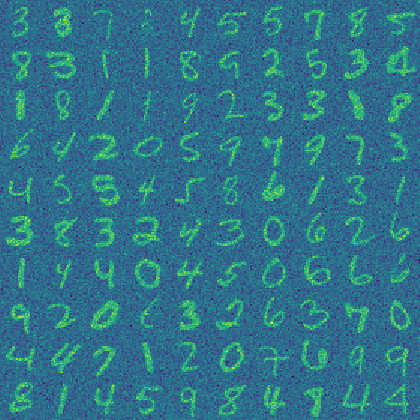
\includegraphics[width=0.3\textwidth]{images/noisy-50.pdf}
 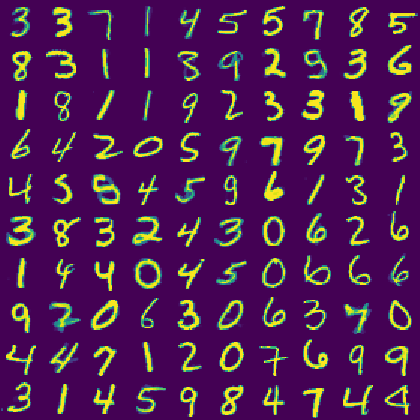
\includegraphics[width=0.3\textwidth]{images/denoised-50-mean.pdf}
 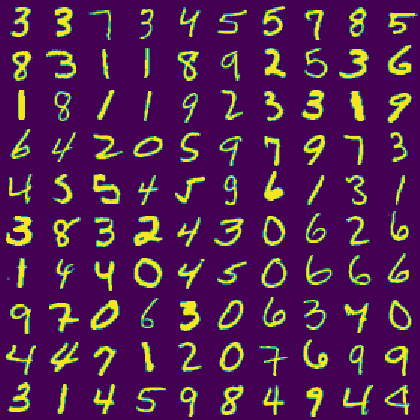
\includegraphics[width=0.3\textwidth]{images/denoised-50-map.pdf}
 \caption{$\sigma$=0.5}
 \label{s5}
\end{figure}

\begin{figure}
 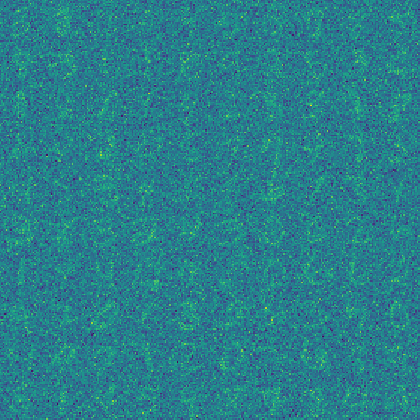
\includegraphics[width=0.3\textwidth]{images/noisy-100.pdf}
 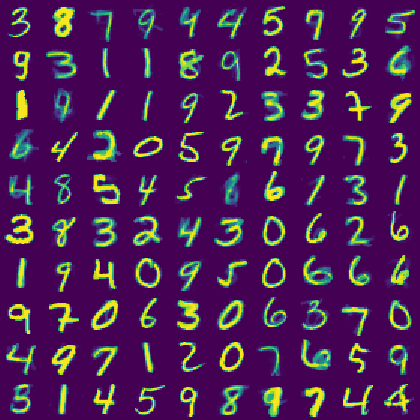
\includegraphics[width=0.3\textwidth]{images/denoised-100-mean.pdf}
 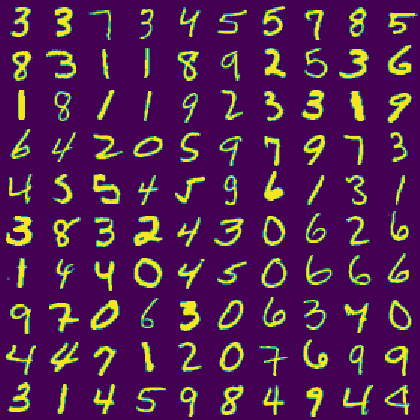
\includegraphics[width=0.3\textwidth]{images/denoised-100-map.pdf}
 \caption{$\sigma$=1}
 \label{s1}
\end{figure}

\end{solution}



\end{document}
